% ============================================================================
% 서울대학교 공학 박사학위논문
% Seoul National University Ph.D. Dissertation
%
% 서울대학교 대학원 학위논문 작성 지침 기반
%   - 판형: 4×6배판 (19cm × 26cm)
%   - 본문: 11pt, 명조체
%   - 여백: 위 20mm, 아래 15mm, 왼쪽 30mm, 오른쪽 30mm
%   - 머리말 15mm, 꼬리말 15mm
%   - 줄간격: 170% 이상
%
% 작성: 박세용 (Saeyong Park)
% 최초 작성: 2026-04
% ============================================================================

\documentclass[11pt]{report}

% ── 판형 설정 (4×6배판: 19cm × 26cm) ──────────────────────────────────────
\usepackage[
  paperwidth=190mm,
  paperheight=260mm,
  top=20mm,
  bottom=15mm,
  left=30mm,
  right=30mm,
  headheight=15mm,
  headsep=5mm,
  footskip=15mm
]{geometry}

% ── 패키지 ──────────────────────────────────────────────────────────────────
\usepackage[T1]{fontenc}
\usepackage{kotex}                  % 한국어
\usepackage{times}                  % Times New Roman (영문 명조)
\usepackage{amsmath,amssymb,amsfonts}
\usepackage{graphicx}
\usepackage{booktabs}
\usepackage{multirow}
\usepackage{array}
\usepackage{subcaption}
\usepackage{hyperref}
\usepackage{xcolor}
\usepackage{natbib}                 % 참고문헌
\usepackage{algorithm}
\usepackage{algorithmic}
\usepackage{setspace}
\usepackage{fancyhdr}
\usepackage{tocloft}                % TOC 스타일
\usepackage{etoolbox}
\usepackage{emptypage}              % 빈 페이지 헤더 제거

% ── 줄간격 (SNU 기준: 170% 이상) ───────────────────────────────────────────
\setstretch{1.7}

% ── 한글 폰트 설정 ────────────────────────────────────────────────────────────
% kotex 기본(바탕체) 사용; XeLaTeX 컴파일 시 \setmainhangulfont{} 으로 변경 가능

% ── 헤더/푸터 ─────────────────────────────────────────────────────────────────
\pagestyle{fancy}
\fancyhf{}
\fancyhead[R]{\thepage}
\fancyhead[L]{\leftmark}
\renewcommand{\headrulewidth}{0.4pt}

% ── 목차 스타일 ───────────────────────────────────────────────────────────────
\renewcommand{\contentsname}{목\quad 차}
\renewcommand{\listfigurename}{그림 목차}
\renewcommand{\listtablename}{표 목차}
\renewcommand{\bibname}{참고문헌}

% ── 그림/표 번호 (chapter.number 형식) ───────────────────────────────────────
\numberwithin{equation}{chapter}
\numberwithin{figure}{chapter}
\numberwithin{table}{chapter}

% ── hyperref 설정 ─────────────────────────────────────────────────────────────
\hypersetup{
  colorlinks=true,
  linkcolor=black,
  citecolor=blue,
  urlcolor=blue,
  pdftitle={선박 탑재 LiDAR 기반 실시간 파랑장 추정과 그 제어 응용},
  pdfauthor={박세용},
}

% ── 단축 명령어 ───────────────────────────────────────────────────────────────
\newcommand{\Hs}{H_{\mathrm{s}}}
\newcommand{\Tp}{T_{\mathrm{p}}}
\newcommand{\nRMSE}{\text{nRMSE}}
\newcommand{\disp}{\mathrm{disp}}
\newcommand{\WS}{\textsc{WaveSplat}}
\newcommand{\todo}[1]{\textcolor{red}{[TODO: #1]}}

% ============================================================================
\begin{document}

% ── 페이지 번호 로마자 (표지 ~ 목차) ─────────────────────────────────────────
\pagenumbering{roman}
\setcounter{page}{1}

% ============================================================================
% 표지 (Cover Page)
% ============================================================================
\begin{titlepage}
\thispagestyle{empty}
\begin{center}

\vspace*{2cm}

{\Large \textbf{공학박사 학위논문}}

\vspace{2cm}

{\LARGE \textbf{선박 탑재 LiDAR 기반 실시간 파랑장 추정과\\[0.3em] 그 제어 응용}}

\vspace{1cm}

{\large \textbf{Real-Time Ocean Wave Field Estimation from\\[0.3em]
Shipboard LiDAR and Its Control Applications}}

\vspace{3cm}

{\large 2026년 \quad 월}

\vspace{2cm}

{\large 서울대학교 대학원}\\[0.5em]
{\large 조선해양공학과}

\vspace{1.5cm}

{\large 박\quad 세\quad 용}

\end{center}
\end{titlepage}

% ============================================================================
% 인준지 (Approval Page)
% ============================================================================
\newpage
\thispagestyle{empty}
\begin{center}

\vspace*{2cm}

{\large \textbf{선박 탑재 LiDAR 기반 실시간 파랑장 추정과 그 제어 응용}}

\vspace{1cm}

{\large 지도교수 \quad \todo{지도교수 성함}}

\vspace{1cm}

{\large 이 논문을 공학박사 학위논문으로 제출함}

\vspace{0.5cm}

{\large 2026년 \quad 월 \quad 일}

\vspace{1.5cm}

{\large 서울대학교 대학원}\\[0.5em]
{\large 조선해양공학과}

\vspace{0.5cm}

{\large 박\quad 세\quad 용}

\vspace{2cm}

{\large 박세용의 공학박사 학위논문을 인준함}

\vspace{0.5cm}

{\large 2026년 \quad 월 \quad 일}

\vspace{1.5cm}

\begin{tabular}{rl}
위원장 & \underline{\hspace{6cm}} \\[1.2em]
부위원장 & \underline{\hspace{6cm}} \\[1.2em]
위\quad 원 & \underline{\hspace{6cm}} \\[1.2em]
위\quad 원 & \underline{\hspace{6cm}} \\[1.2em]
위\quad 원 & \underline{\hspace{6cm}} \\
\end{tabular}

\end{center}

% ============================================================================
% 국문초록
% ============================================================================
\newpage
\chapter*{초\quad 록}
\addcontentsline{toc}{chapter}{초\quad 록}

선박 탑재 스캐닝 LiDAR는 전방 해수면을 10\,Hz로 스캔하여 프레임당 약 50--200개의
3차원 관측점을 생성한다. 이러한 희소하고 불균질한 관측으로부터
연속적이고 물리적으로 타당한 파도장을 실시간으로 복원하는 것은,
자율운항 선박의 안전·승차감·에너지 효율 향상과
파랑 예측 기반 제어 응용을 위한 핵심 기술 과제이다.

기존의 격자 기반 방법(Ensemble Transform Kalman Filter, ETKF)은
희소 관측을 공간 격자에 보간하는 과정에서 aliasing이 발생하고,
격자 해상도와 앙상블 크기에 따른 높은 계산 비용과 민감한 하이퍼파라미터 조정이
요구된다는 근본적 한계를 가진다.
Gaussian Process Regression (GPR)은 격자 없이 공간 보간을 수행할 수 있으나
$\mathcal{O}(M^3)$ 계산 복잡도와 시간 모델의 부재로 인해
실시간 추적에 한계가 있으며, 6-지표 패널 평가에서 near-zero predictor로 진단된다.

본 논문은 격자를 사용하지 않는(grid-free) 스펙트럼 Gaussian 파면 표현에 기반한
실시간 파도장 추정 알고리즘 \WS{}를 제안한다.
파도장을 $N$개의 평면파(plane wave) 집합으로 직접 파라미터화하고,
각주파수를 선형 분산관계
$\omega_i = \sqrt{g|k_i|\tanh(|k_i|d)}$로 구속함으로써
자유 파라미터를 $5N$에서 $4N$으로 감소시킨다.
입사각과 거리에 의존하는 Fresnel 신뢰 가중치를 도입하여
LiDAR 관측 품질의 공간적 불균질성을 직접 모델링한다.
또한 에너지 기반 가지치기(pruning)와 잔차 기반 성장(growth)을 통해
파도 성분 수 $N$을 관측된 해상(海象) 복잡도에 자동 적응시킨다.

100개 에피소드(Beaufort 2--5 해상, 성분 수 1--30, 5개 시드, 2가지 raydrop 모델)에
걸친 평가에서, \WS{}는 하이퍼파라미터를 최적화한 ETKF 대비 평균 nRMSE를
\textbf{30.1\%} 낮추고 (\textbf{0.223} vs.\ \textbf{0.319}),
처리 속도는 약 \textbf{10배} 빠른 \textbf{13.4\,ms/프레임}을 달성한다.
사전 등록된 6개 지표 평가 패널에서 \WS{}는 zero-predictor 대비 양수의
Skill Score를 기록한 유일한 방법임을 보인다.
100회 대응 검증을 통한 Wilcoxon signed-rank 검정 결과
($p = 1.1\times10^{-15}$, Cohen's $d = 1.16$)는 이 차이가
통계적으로 매우 유의미한 large effect임을 확인한다.

또한 본 논문은 \WS{}의 downstream 응용으로서,
추정된 파랑 정보를 활용한 하이드로포일 선박의 2자유도 feedforward 제어
알고리즘을 제안하고 시뮬레이션을 통해 검증한다.
Tandem-foil 하이드로포일 선박(1700\,kg, 22\,knots)에 대해
PD 피드백 위에 파랑 미리보기(wave preview) feedforward를 추가하여,
Beaufort 3--4 조건에서 수직 가속도 RMS를 \textbf{11--41\%} 감소시킨다.
End-to-end 검증에서 \WS{} 기반 feedforward는 완벽한 파도 정보 대비
Beaufort 3에서 \textbf{92--96\%}의 성능을 달성하며,
ISO 2631 승차감 등급을 ``Slight discomfort''에서 ``Comfortable''로 개선한다.
민감도 분석에서 feedforward는 50\% nRMSE까지도 효과적이며,
최적 미리보기 거리는 0.1--0.3초(1--3\,m)임을 확인한다.

\vspace{1em}
\noindent\textbf{주요어:} 파도장 추정, 선박 탑재 LiDAR, 스펙트럼 방법,
분산관계, 격자 비의존 표현, 실시간 추정, 하이드로포일, feedforward 제어,
파랑 미리보기

\noindent\textbf{학번:} \todo{학번}

% ============================================================================
% 영문초록
% ============================================================================
\newpage
\chapter*{Abstract}
\addcontentsline{toc}{chapter}{Abstract}

Shipboard scanning LiDAR generates approximately 50--200 three-dimensional
observation points per frame by scanning the forward ocean surface at 10\,Hz.
Recovering a continuous, physically valid wave field from these sparse and
heterogeneous observations in real time is a critical enabling technology for
autonomous vessel safety, ride comfort, and energy efficiency, as well as for
wave-preview control applications.

Existing grid-based methods such as the Ensemble Transform Kalman Filter
(ETKF) suffer from aliasing introduced by interpolating sparse observations
onto regular grids, high computational cost proportional to grid resolution
and ensemble size, and sensitivity to hyperparameter tuning.
Gaussian Process Regression (GPR) avoids gridding but has $\mathcal{O}(M^3)$
complexity and lacks a temporal propagation model, functioning as a near-zero
predictor in multi-metric evaluation.

This dissertation proposes \WS{}, a real-time ocean wave field estimation
algorithm based on a grid-free spectral Gaussian wave field representation.
The wave field is directly parameterized as a superposition of $N$ plane
waves, with angular frequency constrained by the linear dispersion relation
$\omega_i = \sqrt{g|k_i|\tanh(|k_i|d)}$, reducing free parameters from $5N$
to $4N$. A Fresnel-zone confidence weighting scheme explicitly models the
spatially heterogeneous quality of LiDAR observations as a function of
incidence angle and range. An energy-based pruning and residual-triggered
growth mechanism adapts the number of wave components $N$ to the observed
sea state complexity.

On a dataset of 100 episodes spanning Beaufort 2--5 sea states
(1--30 wave components, 5 random seeds, 2 raydrop models), \WS{} achieves a
\textbf{30.1\%} lower average nRMSE than a hyperparameter-tuned ETKF-grid
baseline (\textbf{0.223} vs.\ \textbf{0.319}) while running approximately
\textbf{10$\times$} faster (\textbf{13.4\,ms/frame}).
A pre-registered six-metric evaluation panel shows that \WS{} is the only
method with a positive Skill Score against a zero predictor.
A 100-paired-run statistical validation confirms this improvement is highly
significant ($p = 1.1\times10^{-15}$, Wilcoxon signed-rank;
Cohen's $d = 1.16$, large effect).

This dissertation further presents a downstream application of \WS{}: a
two-degree-of-freedom feedforward control algorithm for hydrofoil vessels
that leverages estimated wave field information for wave-preview ride comfort
improvement. For a tandem-foil hydrofoil vessel (1700\,kg, 22\,knots),
adding wave-preview feedforward to PD feedback reduces heave acceleration
RMS by \textbf{11--41\%} across Beaufort 3--4 scenarios.
In the end-to-end pipeline, \WS{}-based feedforward achieves
\textbf{92--96\%} of perfect-knowledge performance in Beaufort 3, improving
ISO 2631 comfort from ``Slight discomfort'' to ``Comfortable.''
Sensitivity analysis demonstrates that feedforward remains beneficial up to
50\% nRMSE and that the optimal preview horizon is 0.1--0.3\,s.

\vspace{1em}
\noindent\textbf{Keywords:} wave field estimation, shipboard LiDAR, spectral
methods, dispersion relation, grid-free representation, real-time estimation,
hydrofoil, feedforward control, wave preview

\noindent\textbf{Student Number:} \todo{student number}

% ============================================================================
% 목차 / 그림 목차 / 표 목차
% ============================================================================
\newpage
\tableofcontents

\newpage
\listoffigures

\newpage
\listoftables

% ============================================================================
% 본문 시작 — 아라비아 숫자 페이지 번호
% ============================================================================
\newpage
\pagenumbering{arabic}
\setcounter{page}{1}

% ============================================================================
% 제1장. 서론
% ============================================================================
\chapter{서론}
\label{chap:intro}

\section{연구 배경 및 동기}
\label{sec:motivation}

해양 파도장에 대한 실시간 정보는 자율운항 및 반자율운항 선박의 다양한 기능에
필수적이다~\citep{DeanDalrymple1991}.
단기 파랑 예측을 통한 화물 하역 및 헬리콥터 착함 시 선제적 운동 보상,
연료 소비와 구조 피로 하중을 최소화하는 항로 최적화,
고속 하이드로포일 선박의 파랑 미리보기(wave preview) feedforward 제어를
통한 승차감 향상, 그리고 구조 건전성 모니터링 등이 대표적 응용이다.
이 모든 응용에서 파도장 추정치의 공간 해상도, 갱신 속도, 정확도가
해당 기능의 성능을 결정한다.

센서 측면에서, wave buoy는 단일 점에서의 시계열만 제공하여 공간 분포를 알 수 없고,
X-band 해상 레이더~\citep{Drazen2008}는 넓은 관측 범위를 제공하나 산란 강도를
측정하므로 파고 직접 관측이 불가능하며, 위성 고도계는 킬로미터 규모의 해상도와
비실시간 특성으로 선박 규모 실시간 사용에 부적합하다.
이에 비해 선박 탑재 스캐닝 LiDAR는 전방 해수면을 비접촉으로 직접 관측할 수 있는
실용적 센서로, 10\,Hz의 스캔 속도와 250\,m 이상의 관측 거리에서
센티미터 수준의 근거리 정밀도를 제공한다.
최신 solid-state LiDAR (예: Seyond Falcon K1, 1550\,nm, 152채널,
수평 FOV $120^\circ$, 수직 FOV $25^\circ$)의 발전으로 실용화 단계에
진입하고 있다~\citep{SeyondFalconK1}.

그러나 LiDAR 관측은 본질적으로 희소(sparse)하고 불균질하다.
고정 각도 분해능에 의해 근거리는 조밀하고 원거리는 희박한 관측 패턴을 생성하며,
빔 발산(beam divergence)과 해수면 specular reflection에 의한 raydrop,
그리고 grazing angle에서의 Fresnel 반사율 증가에 따른 신호 손실이 존재한다.
프레임당 유효 관측점 수는 해상 상태, 선박 운동, LiDAR raydrop 특성에 따라
50--200개로 변동한다.
이러한 희소하고 불균질한 관측으로부터 연속적인 파도장을
복원하는 것이 본 논문이 다루는 핵심 문제이다.

특히 하이드로포일 선박의 경우, 파랑 미리보기 정보를
feedforward 제어에 활용하면 반응형 제어(reactive control) 대비
현저히 향상된 승차감을 달성할 수 있다.
하이드로포일은 얕은 침수 깊이(0.5--1.0\,m)에서 운용되어
파랑 유기 받음각(angle of attack) 섭동에 매우 민감하므로,
피드백 제어만으로는 파도 교란의 초기 가속도 피크를 방지할 수 없다.
파도장 추정 결과를 활용한 feedforward 보상은 이 인과적 한계를 극복하는
유망한 접근법이다.

\section{기존 연구의 한계}
\label{sec:prior_limitations}

기존의 선박 탑재 LiDAR 기반 파도장 추정 연구는 크게 세 가지 범주로 분류된다.

\paragraph{격자 기반 방법 (Grid-based methods)}
Ensemble Transform Kalman Filter (ETKF)~\citep{Desmars2020, Huhn2022}는
파도장을 공간 격자 위에서 앙상블 상태로 추정하는 데이터 동화 방법이다.
\citet{Desmars2020}이 X-band 레이더로부터의 ETKF 기반 재구성을 최초 제안하고,
\citet{Huhn2022}가 LiDAR 관측으로 확장하였다.
이 접근법은 원칙적으로 견고하나, 희소 LiDAR 관측에 적용 시 세 가지 근본적 한계가 있다:
(i) 희소 관측을 격자에 보간하는 과정에서의 \emph{aliasing} --- 5\,m 격자는
LiDAR 밀도와 무관하게 $\sim$10\,m 이하 파장을 해석할 수 없다;
(ii) 해상 복잡도와 무관한 \emph{고정 해상도} --- 단순한 해상에서는
표현 용량이 낭비되고, 복잡한 해상에서는 해상도가 부족하다;
(iii) \emph{계산 비용} $\mathcal{O}(N_e G^2 \log G^2)$ --- 격자 크기 $G^2$와
앙상블 크기 $N_e$의 곱에 비례하여 실시간 운용이 제한된다.

\paragraph{격자 비의존 공간 보간법}
Gaussian Process Regression (GPR)~\citep{RasmussenWilliams2006}은
Mat\'{e}rn 또는 squared-exponential 커널을 사용한 비모수적 공간 보간으로
격자 없이 파도장을 추정할 수 있다. 그러나 $\mathcal{O}(M^3)$ Cholesky
분해 비용으로 관측점 수 $M$이 증가하면 계산이 비실용적이 되고(프레임당 200\,ms 초과),
표준 형태에서는 시간 전파 모델이 없어 프레임 간 연속성을 보장하지 못한다.
Sparse approximation~\citep{RasmussenWilliams2006}은 비용을 완화하나,
파도장을 분산관계를 만족하는 전파 신호가 아닌 일반적 공간 랜덤 프로세스로
취급하는 근본적 한계가 남는다.

\paragraph{학습 기반 방법}
물리 정보 신경망(PINN)~\citep{Zhang2022}, Fourier Neural Operator
(FNO)~\citep{Ehlers2024}, 비선형 ETKF 확장~\citep{Desmars2024} 등의
학습 기반 방법이 제안되었다. 이들은 학습 분포에서 우수한 성능을 보이나,
FNO 등은 균일 격자를 가정하여 LiDAR의 불규칙 샘플링 패턴과 호환이 어렵고,
센서 형상 간 일반화가 제한적이며, black-box 특성으로 장애 진단이 곤란하다.

이 세 범주의 방법 모두 선박 탑재 LiDAR의 핵심 특성 --- 관측의 공간적 불균질성,
입사각·거리 의존 노이즈, 실시간 제약 --- 을 동시에 충분히 다루지 못한다.

\section{연구 목적 및 기여}
\label{sec:contributions}

본 논문의 목적은 희소 선박 탑재 LiDAR 관측으로부터
물리적으로 타당하고 계산 효율적인 실시간 파도장 추정 방법을 개발하고,
이를 하이드로포일 선박의 파랑 예측 기반 제어에 응용하는 것이다.

본 논문의 주요 기여는 다음과 같다:

\begin{enumerate}
  \item \textbf{격자 비의존 스펙트럼 Gaussian 파면 추정 프레임워크 (\WS{})}: \\
        3D Gaussian Splatting~\citep{Kerbl2023}의 아이디어를 해양 파면 추정에
        최초로 적용하여, 파도장을 $N$개의 평면파 집합으로 직접 파라미터화한다.
        격자 보간 없이 희소·불규칙 관측에서 직접 추정하며,
        분산관계 기반 위상 전파를 통해 프레임 간 시간 추적을 수행한다.

  \item \textbf{분산관계 하드 제약}: \\
        각주파수를 $\omega_i = \sqrt{g|k_i|\tanh(|k_i|d)}$로 구속하여
        자유 파라미터를 $5N \to 4N$으로 감소시키고 물리적 유효성을 보장한다.
        이 제약은 추적 단계에서 위상 예측의 warm start를 제공하여
        프레임당 최적화 스텝을 200회에서 10회로 감소시킨다.

  \item \textbf{Fresnel 신뢰 가중치}: \\
        LiDAR 관측의 입사각·거리 의존 품질을 직접 모델링하여,
        관측 품질이 공간적으로 크게 변하는 해양 표면 측정의
        이분산성(heteroscedasticity)을 반영한다.

  \item \textbf{적응형 성분 수 ($N$) 제어}: \\
        에너지 기반 가지치기와 잔차 기반 성장을 통해
        단순 너울($N=1$)부터 복잡한 다성분 해상($N=21$)까지
        해상 복잡도에 자동 적응한다.

  \item \textbf{사전 등록 6-지표 평가 패널}: \\
        nRMSE 단일 지표로는 걸러낼 수 없는 zero-predictor를 진단하는
        6개 지표(nRMSE, VR, $\rho$, SS, Dir $R^2$, $H_s$ error)를
        사전 등록하여 공정한 비교를 수행한다.

  \item \textbf{공정한 ETKF 기준선}: \\
        24개 설정 하이퍼파라미터 스윕을 통해 최적화된 ETKF를
        기준선으로 제공하여, 임의의 파라미터 선택에 따른 불이익을 방지한다.

  \item \textbf{파랑 예측 기반 하이드로포일 2DOF feedforward 제어}: \\
        \WS{}의 파도장 추정 결과를 활용하는 downstream 제어 응용을 제시한다.
        Dual-actuator feedforward 구조, IIR 저역통과 필터 설계,
        추정 오차 허용 범위 및 최적 미리보기 거리 분석을 포함한다.
\end{enumerate}

\section{논문 구성}
\label{sec:organization}

본 논문의 구성은 다음과 같다.
제2장에서는 해양 파도장 추정과 하이드로포일 제어에 관한 관련 연구를 검토한다.
제3장에서는 \WS{} 알고리즘의 방법론, 시뮬레이션 환경, 실험 설계, 및
실험 결과를 상세히 기술한다.
제4장에서는 하이드로포일 동역학 모델, feedforward 제어 알고리즘, 민감도 분석,
및 end-to-end 검증 결과를 제시한다.
제5장에서는 수조 실험 검증 계획을 다룬다.
제6장에서는 결론과 향후 연구 방향을 논한다.

% ============================================================================
% 제2장. 관련 연구
% ============================================================================
\chapter{관련 연구}
\label{chap:related}

본 장에서는 본 논문의 두 가지 핵심 주제 --- 해수면 파도장 추정과
하이드로포일 선박 제어 --- 에 관한 선행 연구를 검토한다.
관측 센서, 추정 알고리즘, 하이드로포일 동역학 및 제어의 세 축으로 정리한다.

\section{선박 탑재 파랑 관측 센서}
\label{sec:wave_sensing}

해수면 파도장 관측을 위한 선박 탑재 센서는 관측 원리와 공간 분해능에 따라
구분된다. 표~\ref{tab:sensor_comparison}에 주요 센서 모달리티의 정량적 비교를
정리하였다.

\begin{table}[htbp]
\centering
\caption{선박 규모 파도장 추정을 위한 해양 표면 관측 센서 비교.}
\label{tab:sensor_comparison}
\begin{tabular}{lccccl}
\toprule
센서 & 공간 범위 & 해상도 & 갱신 속도 & 직접 파고? & 주요 한계 \\
\midrule
Wave buoy & 점 & --- & 1\,Hz & 예 & 공간 정보 없음 \\
X-band 레이더 & 0.5--4\,km & $\sim$7.5\,m & 1--2\,s & 아니오 & SNR 역변환 필요 \\
위성 고도계 & 전구 & $\sim$7\,km & 수일 & 예 (nadir) & 비실시간 \\
선박 탑재 LiDAR & 10--250\,m & $\sim$0.1\,m & 10\,Hz & 예 & 희소, 거리 의존 노이즈 \\
선박 운동 (RAO) & --- & --- & 연속 & 간접 & 조우파만 추정 \\
\bottomrule
\end{tabular}
\end{table}

\textbf{X-band 해상 레이더}는 선박 탑재 파도 관측에서 가장 광범위하게 연구된 센서이다.
Young~(1985)이 레이더 후방산란 변조(tilt, hydrodynamic, shadowing)에
파도 스펙트럼 정보가 포함됨을 최초로 입증하였고,
Nieto Borge et al.~(2004)가 $(k_x, k_y, \omega)$ 3D FFT와
선형 분산관계를 스펙트럼 필터로 활용하여 방향 파도 스펙트럼을 복원하였다.
이 ``분산 필터링'' 개념은 본 논문의 분산관계 제약 파라미터화와 개념적으로
유사하나, Fourier 영역에서의 필터링이 아닌 하드 파라미터 제약으로 적용된다.
레이더의 근본적 한계는 산란 강도를 측정하므로 경험적 변조 전달 함수(MTF)가
필요하다는 점과, $\sim$7.5\,m의 공간 해상도가 LiDAR ($\sim$0.1\,m)보다
두 자릿수 조잡하다는 점이다.

\textbf{선박 운동 기반 방법}은 선박의 Response Amplitude Operator (RAO)를
역변환하여 조우파 스펙트럼을 추정한다.
추가 센서가 불필요하나 방향 파도 스펙트럼만 복원 가능하고,
공간적으로 분해된 파도장을 제공하지 못한다.

\textbf{선박 탑재 스캐닝 LiDAR}는 해수면에 대한 직접적 파고 측정을 제공하며,
근거리에서 센티미터 수준의 정밀도를 달성한다.
현대의 solid-state LiDAR 기술의 발전으로 소형화·저가화가 진행되고 있으며,
1550\,nm 파장은 eye-safe 운용이 가능하다.
그러나 LiDAR 관측의 세 가지 특이성 --- (1) 거리 증가에 따른 관측 밀도 감소,
(2) grazing angle에서의 specular reflection에 의한 raydrop,
(3) 해수면의 동적 특성에 의한 관측 노이즈 --- 이 추정 알고리즘 설계에
핵심적 제약을 부과한다. 본 논문에서 이를 Fresnel 신뢰 가중치로 직접 모델링한다.

\section{격자 기반 파도장 추정}
\label{sec:grid_methods}

선박 탑재 LiDAR/레이더로부터의 결정론적 파도장 재구성은
공간 격자 이산화와 앙상블 데이터 동화의 결합으로 지배되어 왔다.
\citet{Desmars2020}이 X-band 레이더 관측으로부터 ETKF 기반 재구성을 제안하였으며,
Ensemble Transform Kalman Filter~(Hunt et al., 2007)는 확률론적
EnKF~(Evensen, 2003)의 결정론적 분석 단계를 제공하여 선호된다.
\citet{Huhn2022}가 이 프레임워크를 LiDAR 관측으로 확장하였고(``from points to
waves''), Desmars et al.~(2023)이 실시간 재구성과 1피크 주기 앞까지의
단기 예측을 시연하였다.

이 격자 기반 방법들은 공통 구조 --- 2D 영역을 정규 격자로 이산화하고,
스펙트럼 상태의 앙상블을 유지하며, Kalman update로 관측을 동화 --- 를 공유한다.
이 구조는 공간 해상도와 계산 비용 간의 본질적 trade-off를 수반하며,
희소 관측에서 격자점으로의 보간이 알려진 오차 원천이다.
본 논문에서는 24개 설정의 하이퍼파라미터 스윕을 통해 최적화된 ETKF를
공정한 기준선으로 제공한다 (제3장 \S\ref{sec:baselines}).

\section{격자 비의존 및 스펙트럼 방법}
\label{sec:gridfree_methods}

격자 기반 동화의 대안으로 여러 접근법이 탐색되었다.

고전적 \textbf{스펙트럼 추정} 방법(FFT, Welch, MUSIC, ESPRIT)은
정규 샘플링을 가정한다. Capon의 minimum-variance 빔포밍과
MUSIC은 불규칙 어레이를 처리할 수 있으나, 파워 스펙트럼만 제공하거나(Capon)
모델 차수를 사전에 알아야 한다(MUSIC).
\WS{}는 빔포밍을 \emph{초기화}에만 활용하고, 물리 제약 하의 경사 최적화로
진폭-위상을 동시 복원하여, 빔포밍의 견고성과 완전한 파동 파라미터 복원을 결합한다.

\textbf{GPR}~\citep{RasmussenWilliams2006}은 비모수적 공간 보간을 제공하나,
$\mathcal{O}(M^3)$ 비용과 시간 모델 부재가 근본적 한계이다.
본 논문의 6-지표 평가에서 GPR은 variance ratio = 0.065 (진폭의 6.5\%만 재현)로
near-zero predictor의 진단적 특성을 보인다.

\textbf{학습 기반 방법}으로는 PINN~\citep{Zhang2022}에 의한 파동 방정식
제약 재구성, FNO~\citep{Ehlers2024}에 의한 위상 분해 재구성,
비선형 ETKF 확장~\citep{Desmars2024} 등이 있다.
이들은 학습 분포에서 우수한 결과를 보이나,
FNO의 균일 격자 가정은 LiDAR의 불규칙 샘플링과 비호환적이고,
센서 형상 간 일반화가 제한적이며, black-box 특성이 장애 진단을 어렵게 한다.

\WS{}는 이와 대조적으로 학습 데이터가 필요 없고, 불규칙 관측 형상을 자연스럽게
처리하며, 분산관계를 구조적으로 만족하는 직접 해석 가능한 스펙트럼 파라미터를 생성한다.
격자 비의존 희소 표현은 compressed sensing~(Cand\`{e}s et al., 2006)과
\citet{Drazen2008}의 압력 센서 기반 희소 스펙트럼 재구성과 개념적으로 관련되나,
(1) 각 기저 함수가 물리적 의미의 평면파인 점과
(2) 모델 차수가 잔차 에너지에 기반하여 온라인으로 적응하는 점에서 차별화된다.

\section{하이드로포일 선박 동역학 및 제어}
\label{sec:hydrofoil_control}

\subsection{하이드로포일 역학}

하이드로포일 선박은 수중 양력 날개(foil)로 선체를 수면 위로 들어올려
선체 조파 저항을 제거하고 총 항력을 배수량형 선박 대비 40--60\% 감소시킨다.
1950--70년대에 군사·제한적 상업 용도로 개발되었으며,
전기 추진과의 결합으로 zero-emission 고속 여객 페리가 가능해지면서 재조명되고 있다.

Foilborne 모드의 핵심 특성은 수직 안정성이 전적으로
foil의 양력 기울기(lift-slope) 특성에 의존한다는 점이다.
배수량형 선박의 수선면적 기반 정수력학적 복원력과 달리,
foil의 받음각(AoA) 변화에 따른 양력 변동이 직접적으로
heave와 pitch 가속도를 유발한다.
Beaufort 3(해안 하이드로포일 노선의 일반적 운항 한계)에서
제어되지 않은 수직 가속도는 1\,m/s$^2$를 초과하여
ISO 2631의 ``Fairly uncomfortable'' 범위에 해당한다.

파도 조우 주파수(encounter frequency)는 제어 설계의 핵심 파라미터이다.
속도 $V$로 파도 방향 $\beta$에 대해 운항하는 선박이 주파수 $\omega_0$의
파도를 만나면, 조우 주파수는
$\omega_e = \omega_0 - \omega_0^2 V \cos\beta / g$이다.
22 knots에서 BF3 head sea ($T_p = 5$\,s) 기준, $\omega_e \approx 3.1$\,rad/s
($T_e \approx 2.0$\,s)로 실제 파도 주파수의 2배 이상이 되어,
하이드로포일 제어는 해상 상태가 시사하는 것보다 높은 주파수를 다루어야 한다.

\subsection{능동 승차감 제어}

고속 해양 선박의 능동 승차감 제어는 1990년대 이후 광범위하게 연구되었다.
Haywood et al.~(1995)는 T-foil과 trim tab을 사용한 고속 페리(40--50\,m급)의
PID 피드백 제어를 개발하여 head sea에서 30--50\% 운동 저감을 시연하였다.
Giron-Sierra et al.~(2001)는 fin과 T-foil의 다중 액추에이터 제어에서
heave와 pitch 제어 채널을 분리하는 collective--differential 제어 분해를 도입하였다.
Esteban et al.~(2005)는 strip theory 기반 고속 선박 모델링에서
pitch 제어에 전후 제어면의 차동 구동이 필요함을 보였다.

이 모든 선행 연구는 순수 피드백 제어를 사용하며,
파랑 미리보기 정보를 feedforward 보상에 활용하지 않는다.
피드백 제어의 근본적 한계는 인과적 제약(causal constraint)으로,
파도 교란이 이미 선박에 영향을 미친 후에만 대응할 수 있다는 점이다.
빠른 센서(100\,Hz IMU)와 액추에이터($>$5\,Hz 대역폭)를 사용하더라도
총 루프 지연은 50--100\,ms에 달하며, 이 기간 동안 승객은
파도 유기 가속도 피크를 그대로 경험한다.

\subsection{Model Predictive Control (MPC)}

MPC는 해양 선박 운동 제어에 여러 맥락에서 적용되었다.
P\'{e}rez~(2012)는 fin 기반 선박 롤 안정화에 MPC를 적용하여
제약 처리와 다목적 최적화를 시연하였고,
파력 발전기(WEC)에서는 파랑 미리보기 MPC로 근최적 에너지 추출이 달성되었다.
그러나 하이드로포일 제어에 MPC가 적용된 사례는 없으며,
이는 foilborne 동역학에 필요한 높은 갱신 속도(100\,Hz)와
온라인 최적화의 계산 비용에 기인한다.

본 논문의 feedforward 접근법은 MPC의 간소화된 대안으로 볼 수 있다:
온라인 최적화 문제를 풀지 않고, 예측된 교란에 비례 이득과 저역통과 필터링을
적용한다. 이 간소화는 고려하는 운용 영역에서 파도 유기 AoA와 최적 플랩 보정 간의
근사 선형 관계에 의해 정당화된다.

\subsection{파랑 미리보기 제어}

선박 전방 파도 측정을 feedforward 제어에 활용하는 개념은
자동차 미리보기 서스펜션에 기원을 둔다~(Hrovat, 1997).
해양 분야에서는 주로 파력 발전기와 선박 운동 예측에 탐색되었으며,
Cummins et al.~(2017)이 레이더/LiDAR 기반 파도 미리보기가 단기 선박 운동
예측을 개선함을 보였다.
그러나 실시간 파도장 추정과 선박 운동 제어의 통합은
하이드로포일 선박에서 시연된 바 없다.
하이드로포일의 얕은 침수 깊이가 파도 파고/기울기와 foil 힘 간의
직접적·거의 선형적 결합을 만들어 feedforward 보상에 특히 적합함에도 불구하고이다.

% ============================================================================
% 제3장. 격자 비의존 스펙트럼 파면 추정: WaveSplat
% ============================================================================
\chapter{격자 비의존 스펙트럼 파면 추정: \WS{}}
\label{chap:wavesplat}

% 본 챕터의 내용은 다음 논문을 기반으로 함:
%   S. Park, "WaveSplat: Grid-Free Spectral Wave Field Estimation
%   from Sparse Shipboard LiDAR," Ocean Engineering, 2026 (under review).
% Elsevier 저작권 정책에 따라 학위논문 수록 허용됨.

\section{Forward 모델}
\label{sec:forward}

파도장을 $N$개의 spectral Gaussian(평면파) 집합으로 표현한다:
\begin{equation}
  z(\mathbf{x}, t) = \sum_{i=1}^{N}
    w_i \cos\!\left(k_{x,i} x + k_{y,i} y - \omega_i t + \phi_i\right),
  \label{eq:forward}
\end{equation}
여기서 $w_i$는 진폭, $(k_{x,i}, k_{y,i})$는 파수 벡터,
$\omega_i$는 각주파수, $\phi_i$는 위상이다.
각 성분 $i$는 4개의 자유 파라미터 $(w_i, k_{x,i}, k_{y,i}, \phi_i)$를 가진다.

\paragraph{분산관계 하드 제약}
각주파수는 유한 수심 선형 분산관계에 의해 파수로부터 결정적으로 계산된다:
\begin{equation}
  \omega_i = \sqrt{g |k_i| \tanh(|k_i| d)}, \quad |k_i| = \sqrt{k_{x,i}^2 + k_{y,i}^2},
  \label{eq:dispersion}
\end{equation}
여기서 $g = 9.81$\,m/s$^2$는 중력 가속도, $d$는 수심이다.
이 제약은 매 forward 평가마다 강제하여 $5N$개의 자유 파라미터를 $4N$개로 감소시키고,
추정된 파도장이 물리적으로 전파 가능한 중력파임을 보장한다.
심해 극한($|k|d \gg 1$)에서 $\omega = \sqrt{g|k|}$로 환원되며,
천해 극한($|k|d \ll 1$)에서 $\omega = |k|\sqrt{gd}$로 환원된다.

이 선형 forward 모델은 고차 파도 이론(Gerstner wave, 2차 Stokes 등)에 대해
$\mathcal{O}(\epsilon^2)$ 근사이며, 여기서 $\epsilon = |k| \cdot |w|$는 파도 가파름이다.
Beaufort 4에서 전형적 가파름은 $\epsilon \approx 0.05$로,
모델 불일치는 $< 0.25\%$이다.
본 논문에서 고려하는 Beaufort 2--5 범위(비쇄파)에서
선형 모델은 우수한 근사이다.

최적화 파라미터 집합: $\Theta = \{w_i, k_{x,i}, k_{y,i}, \phi_i\}_{i=1}^{N}$.

\section{관측 모델}
\label{sec:observation}

각 LiDAR 스캔 시점 $t$에서, $M$개의 파고 관측
$\{(x_j, y_j, z_j)\}_{j=1}^{M}$이 불규칙한 공간 위치에서 얻어진다.
관측 모델은:
\begin{equation}
  z_j = \sum_{i=1}^{N} w_i \cos(k_{x,i} x_j + k_{y,i} y_j - \omega_i t + \phi_i) + \eta_j
\end{equation}
여기서 $\eta_j$는 관측 노이즈로, 그 분산은 거리와 입사각에 의존한다.
프레임당 유효 관측 수 $M$은 해상 상태, 선박 운동, LiDAR raydrop 특성에 따라
50--200으로 변동한다.

\subsection{Fresnel 신뢰 가중치}
\label{sec:fresnel}

해양 표면에서의 LiDAR 파고 정밀도는 두 가지 물리적 메커니즘에 의해 저하된다:
(1) 빔 발산으로 인한 원거리 footprint 확대, 이로 인한 국소 표면 곡률 평균화;
(2) 높은 입사각(near-grazing)에서 specular reflection 확률 증가로 인한
전신호 손실 또는 파봉(wave crest) 편향 반환.

다음과 같이 관측별 신뢰 가중치를 정의한다:
\begin{equation}
  c_j = \frac{\cos\theta_j}{d_j / d_{\mathrm{ref}}}, \quad d_{\mathrm{ref}} = 125\,\text{m},
  \label{eq:confidence}
\end{equation}
여기서 $\theta_j$는 빔 입사각(국소 표면 법선과 빔 방향으로부터 계산),
$d_j$는 거리, $d_{\mathrm{ref}} = 125$\,m은 최대 LiDAR 사거리의 절반으로
설정한 기준 거리이다.
$\cos\theta_j$는 Lambertian 투영 인자를,
$d_j/d_{\mathrm{ref}}$는 역제곱 거리 감쇠를 근사한 항으로,
가까이 있고 수직에 가까운 관측에 높은 가중치를 부여한다.

\subsection{손실 함수}
\label{sec:loss}

전체 손실 함수는 다음과 같다:
\begin{equation}
  \mathcal{L}(\Theta) = \underbrace{\frac{1}{M}\sum_{j=1}^{M} c_j \bigl(z_j - \hat{z}_j\bigr)^2}_{\text{가중 MSE}}
    + \underbrace{\lambda_1 \sum_{i=1}^{N}|w_i|}_{\text{희소성}}
    + \underbrace{\lambda_s \sum_{i=1}^{N-1}(w_{\sigma(i+1)} - w_{\sigma(i)})^2}_{\text{스펙트럼 평활화}},
  \label{eq:loss}
\end{equation}
여기서 $M$은 프레임당 관측 점 수이고,
$\lambda_1 = 10^{-3}$은 진폭 희소성 정규화(pruning을 위해 무시 가능한 성분을
0으로 구동), $\lambda_s = 10^{-4}$은 스펙트럼 인접 성분 간의 급격한 진폭 변화를
억제하여 JONSWAP 형태와 일관된 매끄러운 스펙트럼 포락선을 유도하는 정규화이다.
$\sigma$는 $|k|$ 순서로의 정렬을 나타낸다.

\section{2단계 추정 파이프라인}
\label{sec:pipeline}

추정은 두 단계로 진행된다: 다중 프레임 관측으로부터 스펙트럼 모델을 확립하는
초기화 단계, 이어서 최소 계산으로 모델을 유지하는 프레임별 추적 단계.
표~\ref{alg:pipeline}에 전체 파이프라인을 요약하였다.

\begin{table}[htbp]
\centering
\caption{\WS{} 추정 파이프라인 알고리즘.}
\label{alg:pipeline}
\begin{tabular}{p{0.90\textwidth}}
\toprule
\textbf{Phase 1: 초기화} (프레임 $1$ -- $T_\text{init}/\Delta t$) \\
\midrule
1. 다중 프레임 관측 $\{(x_j, y_j, z_j, t_j)\}$ 축적 \\
2. 극좌표 파수 격자에서 빔포밍 파워 $P(k_x, k_y)$ 계산 \\
3. $15^\circ$ 각도 억제 기반 greedy 피크 추출 \\
4. 선형 최소제곱으로 진폭/위상 추정 \\
5. Coarse-to-fine 최적화: $N$=3 $\to$ 8 $\to$ 15 \\
\quad --- 각 단계: 200 Adam steps, lr=$5\times 10^{-3}$ \\
6. 에너지 기반 가지치기 (에너지 90\% 기준) \\
7. 안전 검사: $\Delta$RMSE $> 30\%$ 시 rollback \\
8. 잔차 기반 성장: 잔차 RMS $> 0.05$\,m 시 빔포밍 재적용 ($N_{\max} = 30$) \\
\midrule
\textbf{Phase 2: 추적} (이후 각 프레임) \\
\midrule
1. \textbf{예측}: $\phi_i \mathrel{+}= \omega_i \cdot \Delta t$ \\
2. \textbf{갱신}: 슬라이딩 윈도우 ($K_w$=3 프레임)에서 $K$=10 Adam steps \\
\quad --- $(w_i, \phi_i)$만 갱신; $(k_{x,i}, k_{y,i})$는 고정 \\
\quad --- Learning rate: $1\times 10^{-3}$, scheduling 없음 \\
\bottomrule
\end{tabular}
\end{table}

\subsection{Phase 1: 초기화}
\label{sec:init}

첫 $T_{\text{init}} = 2 T_p$ 초의 관측(여기서 $T_p$는 관측 시계열의 주파수에서
추정한 피크 주기)이 주어지면, 3단계 coarse-to-fine 절차를 통해
모든 스펙트럼 파라미터를 동시 최적화한다.

\paragraph{분산 인식 빔포밍}
초기 파수 추정치를 극좌표 파수 격자 스캔으로 얻는다.
격자는 $|k| \in [0.02, 0.50]$\,rad/m
(파장 $\lambda = 2\pi/|k| \in [12.6, 314]$\,m, Beaufort 2--5 범위,
수심 $d=50$\,m)을 64개 반경 $\times$ 128개 방위각 빈으로 분할한다.
반경 범위는 분산관계로 결정된다:
$|k|_{\min} = 0.02$는 BF5 너울($T_p \approx 9$\,s)에,
$|k|_{\max} = 0.50$은 LiDAR 공간 범위($\sim$200\,m)에서
해석 가능한 최단 파장에 대응한다.

각 후보 $(k_x, k_y)$에 대해 $\omega = \sqrt{g|k|\tanh(|k|d)}$를 계산하고
빔포밍 파워를 평가한다:
\begin{equation}
  P(k_x, k_y) = \left| \sum_{j} z_j \, e^{-i(k_x x_j + k_y y_j - \omega t_j)} \right|^2
\end{equation}
여기서 합산은 $T_\text{init}$ 동안 축적된 모든 관측에 대해 수행된다.
분산관계에서 유도된 $\omega$의 사용은 빔포밍이 $(k_x, k_y, \omega)$ 공간의
분산 곡면 위에 있는 물리적 파도 신호만을 자연스럽게 통과시키고
노이즈를 억제하는 효과를 가진다.

$P$의 피크를 greedy로 추출한다: 최대값을 선택한 후
$15^\circ$ 각도 분리 내의 모든 후보를 억제하고 반복한다.
$15^\circ$ 임계값은 같은 파도 성분의 인접 파수 빈 간 중복 계수를 방지하면서,
교차해(crossing seas)를 해석하기에 충분히 좁다.
추출된 각 성분의 초기 진폭과 위상은
축적된 관측을 선택된 파수 기저함수에 선형 최소제곱 투영하여 추정한다.

\paragraph{Coarse-to-fine 최적화}
빔포밍 초기화로부터 시작하여, 3단계($N$=3 $\to$ 8 $\to$ 15)로
스펙트럼 파라미터를 최적화한다.
각 단계에서 Adam optimizer~(Kingma \& Ba, 2015)로 200회 반복한다
(학습률 $\eta = 5 \times 10^{-3}$, $\beta_1 = 0.9$, $\beta_2 = 0.999$).
초기화 단계에서는 파수 $(k_{x,i}, k_{y,i})$도 자유 파라미터이며
(추적 단계와 달리), 분산 제약은 매 forward 평가 시 $\omega_i$를
$(k_{x,i}, k_{y,i})$로부터 재계산하여 정확히 만족시킨다.

\subsection{적응형 모델 차수}
\label{sec:adaptive}

초기화 후 에너지 기반 가지치기를 적용한다.
성분을 에너지 $E_i = w_i^2$ 내림차순으로 정렬하고,
총 에너지 $\sum_i E_i$의 90\%를 포함하는 최소 집합을 유지한다.
JONSWAP 스펙트럼 형상에서 소수의 피크 근방 성분이 대부분의 파도 에너지를 포함하므로
이 기준이 적절하다.

안전 검사: 가지치기 후 RMSE가 가지치기 전 대비 130\%를 초과하면
전체 롤백한다. 이는 유사 에너지의 두 성분이 다른 공간 영역에 기여하는 경우
(예: 교차해) 개별적으로 저에너지로 보이는 상황을 방지한다.

잔차 기반 성장: 가지치기 후 잔차 RMS가 0.05\,m을 초과하면
(미모델링 파도 에너지 존재), 잔차 신호 $r_j = z_j - \hat{z}_j$에 빔포밍을
재적용하여 주도적 잔차 피크를 모델에 추가한다 ($N_{\max}=30$).

\subsection{Phase 2: 추적 (w\_phi 모드)}
\label{sec:tracking}

초기화 이후 10\,Hz 프레임마다 predict--update 순환을 수행한다:

\begin{enumerate}
  \item \textbf{예측 (Predict)}: 분산관계 유도 각주파수로 위상을 전파한다:
    $\phi_i \leftarrow \phi_i + \omega_i \Delta t$,
    여기서 $\Delta t = 0.1$\,s (10\,Hz LiDAR 프레임 속도).
    이 예측은 분산관계를 만족하는 선형 파도장에서 정확하다.

  \item \textbf{갱신 (Update)}: $K_w = 3$ 슬라이딩 프레임 창에서
    $K = 10$회 Adam 스텝 (lr=$1\times 10^{-3}$)으로
    $(w_i, \phi_i)$만 갱신한다.
    파수 $(k_{x,i}, k_{y,i})$는 고정한다 (\texttt{w\_phi} 추적 모드).
\end{enumerate}

추적 시 파수를 고정하는 근거는 두 가지이다:
(1) 단일 프레임에서 파수 추정은 희소 관측의 공간 aliasing으로 ill-conditioned이다
--- LiDAR의 불규칙 샘플링 패턴이 단일 스냅샷에서 파수를 해석하기에 충분한 제약을
제공하지 못하는 반면, 다중 프레임 초기화는 $\sim$20 프레임에 걸친 평균화로
견고한 파수 추정을 제공한다;
(2) 고정 파수 하에서 분산 제약이 강력한 위상 예측 ($\omega \cdot \Delta t$)을
제공하여 warm start로 작용하므로, 프레임당 경사 스텝을 200회(전체 최적화)에서
10회로 감소시킨다.

슬라이딩 윈도우 ($K_w = 3$)는 최근 3 프레임의 관측을 경사 계산에 사용한다.
10\,Hz에서 0.3\,s 구간으로, 고려하는 모든 해상 상태의 피크 주기 $T_p$보다
훨씬 짧아 과도한 지연 없이 단일 프레임 노이즈를 평활화한다.

\section{계산 복잡도}
\label{sec:complexity}

$M$을 프레임당 LiDAR 관측 수, $N$을 스펙트럼 성분 수라 하자.

\begin{figure}[htbp]
\centering
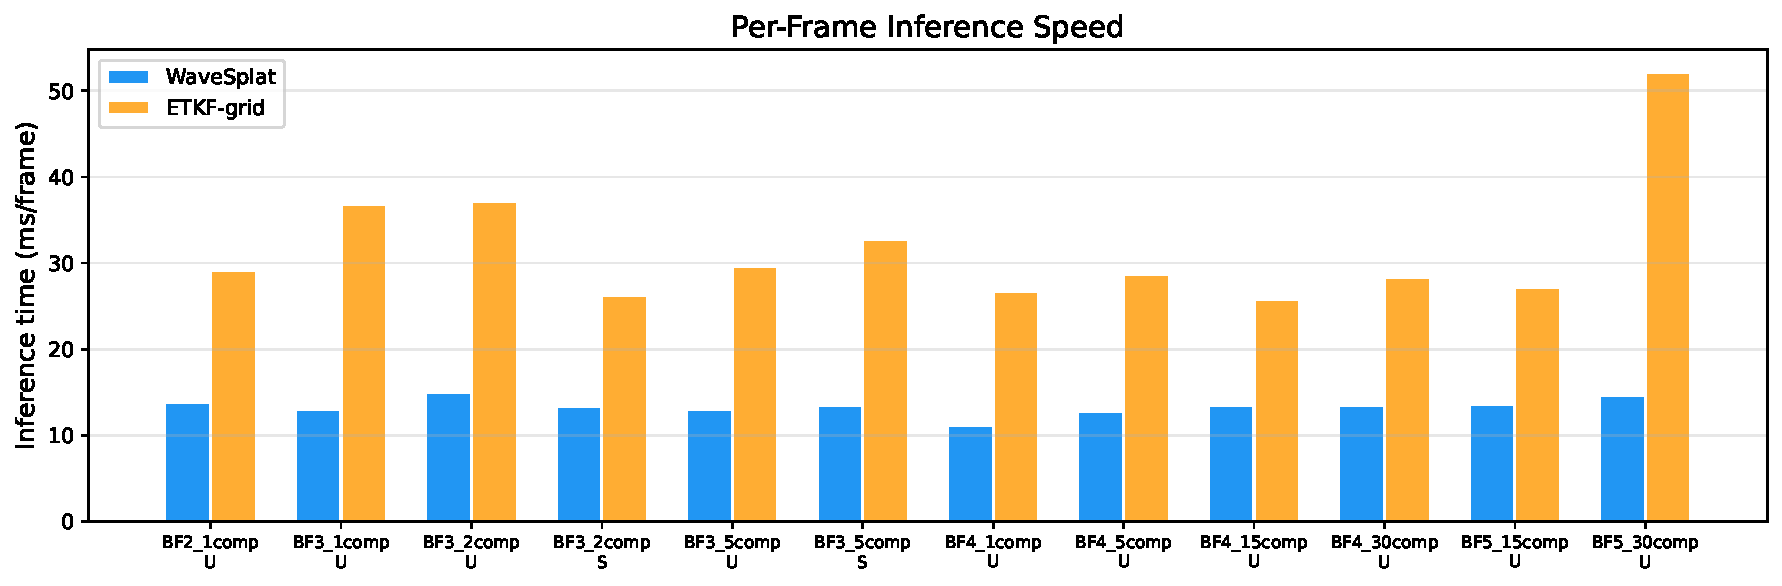
\includegraphics[width=0.80\textwidth]{figures_ws/fig3_speed.pdf}
\caption{프레임당 처리 시간 비교. \WS{}는 13.4\,ms/프레임으로
ETKF (132.6\,ms)와 GPR ($>$200\,ms) 대비 약 10배 이상 빠르며,
10\,Hz LiDAR의 100\,ms 실시간 예산을 충족한다.}
\label{fig:speed}
\end{figure}

\textbf{\WS{}}: 각 forward 평가는
$z(x_j, y_j, t) = \sum_{i=1}^{N} w_i \cos(\cdot)$를 계산하여
프레임당 $\mathcal{O}(M \cdot N)$이다.
$K$ 경사 스텝과 윈도우 크기 $K_w$로 프레임당 추적 비용은
$\mathcal{O}(K \cdot K_w \cdot M \cdot N)$이다.
실제 $K=10$, $K_w=3$, $N \leq 30$에서 CPU 단일 스레드(Intel i7-12700H) 기준
\textbf{13.4\,ms/프레임}.

\textbf{ETKF-grid}: $N_e$개 앙상블 멤버를 $G_x \times G_y$ 격자에 유지.
FFT 기반 전파에 $\mathcal{O}(N_e \cdot G_x G_y \cdot \log(G_x G_y))$,
앙상블 변환에 $\mathcal{O}(N_e^3 + N_e^2 \cdot M)$.
$N_e=100$, $G=40\times30$에서 \textbf{132.6\,ms/프레임}.

\textbf{GPR}: $M$개 관측에 $\mathcal{O}(M^3)$ Cholesky 분해.
50 points/frame에서도 커널 하이퍼파라미터 최적화로 \textbf{$>$200\,ms/프레임}.

\begin{table}[htbp]
\centering
\caption{계산 복잡도 비교. $M$: 관측/프레임, $N$: 스펙트럼 성분,
$G$: 격자 크기, $N_e$: 앙상블 멤버.}
\label{tab:complexity}
\begin{tabular}{lcc}
\toprule
방법 & 프레임당 복잡도 & 실측 \\
\midrule
\WS{} & $\mathcal{O}(K \cdot K_w \cdot M \cdot N)$ & 13.4\,ms \\
ETKF-grid & $\mathcal{O}(N_e \cdot G^2 \log G^2)$ & 132.6\,ms \\
GPR       & $\mathcal{O}(M^3)$ & $>$200\,ms \\
\bottomrule
\end{tabular}
\end{table}

\section{시뮬레이션 환경 (WaveSim)}
\label{sec:wavesim}

물리 기반 LiDAR 파도 시뮬레이션(WaveSim)을 개발하여
ground-truth 파도장과 합성 LiDAR 관측을 생성한다.

\subsection{파도 생성}
\label{sec:wave_gen}

파도장은 JONSWAP 스펙트럼~\citep{Hasselmann1973}으로 파라미터화하고
Gerstner wave~\citep{Gerstner1802}로 생성한다.
Gerstner wave는 2차 비선형 회전파의 정확해로, 수평 궤도 운동(orbital motion)을
포함하여 선형 모델(\ref{eq:forward})의 현실적 테스트를 제공한다.
입자 교차(wave self-intersection) 방지를 위해
Q-제약 $\sum_i Q_i \omega_i A_i \leq 1$을 강제한다.
해상 조건은 Beaufort 2--5 ($H_s = 0.3$--$2.0$\,m, $T_p = 4$--$9$\,s)를 포괄하며,
성분 수 1, 2, 5, 15, 30과 $\pm 20^\circ$ 방향 분산을 포함한다.

\subsection{LiDAR 시뮬레이션}
\label{sec:lidar_sim}

LiDAR 시뮬레이션은 Seyond Falcon K1의 실제 사양을 기반으로 한다:
1550\,nm 파장, 152채널, 수평 FOV $120^\circ$, 수직 FOV $25^\circ$,
500 수평 빔, 10\,Hz 스캔 속도, 사거리 10--250\,m.

Ray-surface 교차는 Möller--Trumbore 알고리즘으로 삼각화된 파면과의
교차점을 정확히 계산한다.
반환 확률은 Fresnel 반사율, 입사각, 거리의 함수로 모델링한다.
Fresnel 반사율은 1550\,nm에서의 해수 복소 굴절률 $n = 1.321$을 사용하며,
입사각이 클수록(grazing) 반사율이 증가하여 specular reflection에 의한
신호 손실(raydrop)이 발생한다.

두 가지 raydrop 모델을 구현하여 LiDAR의 서로 다른 물리적 반환 조건을 모사한다:
\begin{itemize}
  \item \textbf{Uniform (확산 반사)}: $P = \eta \cdot R_\text{Fresnel}(\theta) \cdot \cos\theta / (d/d_\text{ref})^2$
        --- 표면 형상에 독립적인 일정 raydrop 확률
  \item \textbf{Slope (specular backscatter)}: 파면 기울기에 의한 specular backscatter 조건에서만 반환
        --- 급경사 표면에서 높은 raydrop, 파봉 부근에서 높은 반환율
\end{itemize}

시뮬레이션의 물리적 신뢰성은 \textbf{39개의 단위 테스트}로 검증된다:
분산관계 해석해 대비 오차 $< 10^{-6}$\,rad/s,
Gerstner 단일파 RMSE $< 10^{-10}$\,m,
Fresnel 반사율 단조 증가, ray-surface 교차 정밀도, 수심 $d=50$\,m에서의
위상 및 군 속도 일치 등을 포함한다.

\section{실험 설계}
\label{sec:exp_setup}

\subsection{데이터셋}
\label{sec:dataset}

총 100개의 에피소드를 생성한다
(5개 시드 $\times$ 10개 설정 $\times$ 2가지 raydrop 모델).
각 에피소드는 301 프레임 (30\,s, 10\,Hz)으로 구성되며,
ground-truth 파고장은 LiDAR 관측 영역을 포함하는
$80 \times 60$ 공간 격자에서 평가된다.
10개 설정은 Beaufort 2--5 해상($H_s = 0.3$--$2.0$\,m)과
성분 수 1, 2, 5, 15, 30의 조합이다.

\subsection{기준선 방법}
\label{sec:baselines}

\begin{itemize}
  \item \textbf{ETKF (tuned)}: 24개 설정 하이퍼파라미터 스윕에서 최적화된 설정
        --- 격자 해상도 $\{40\times30, 80\times60\}$, 앙상블 크기 $\{50, 100\}$,
        inflation 쌍 $(\alpha, \sigma)$를 탐색하여 최적 설정
        ($g=40\times30$, $N_e=100$, $\alpha=1.0$, $\sigma=0.005$,
        12 sweep 에피소드 평균 nRMSE=0.358)을 선정.
        24개 설정 간 3.3배 편차(0.358 vs.\ 1.187)는
        공정한 ETKF 평가에 튜닝이 필수적임을 확인한다.

  \item \textbf{GPR-1}: 단일 프레임 Mat\'{e}rn $\nu = 5/2$ GPR
        ($\ell = 20$\,m, 노이즈 $\sigma = 0.02$\,m).
        시간 모델이나 물리 제약 없이 순수 공간 보간.

  \item \textbf{GPR-sliding}: 3-프레임 슬라이딩 창 GPR.
        단일 프레임 GPR의 강화 버전으로 시간적 정보를 간접 활용.
\end{itemize}

\begin{table}[htbp]
\centering
\caption{ETKF 하이퍼파라미터 스윕: 24개 설정 중 최상/최하 결과.
$g$=격자 해상도, $n_e$=앙상블 크기, $\alpha$=multiplicative inflation,
$\sigma$=additive inflation. 최상 설정(bold)을 논문 전체에서 ``ETKF (tuned)''로 사용.}
\label{tab:etkf_sweep}
\begin{tabular}{lccccc}
\toprule
& $g$ & $n_e$ & $\alpha$ & $\sigma$ & mean nRMSE \\
\midrule
\textbf{Best (tuned)} & $40\times30$ & 100 & 1.00 & 0.005 & \textbf{0.358} \\
2nd                   & $40\times30$ & 100 & 1.02 & 0.005 & 0.403 \\
3rd                   & $40\times30$ &  50 & 1.00 & 0.005 & 0.416 \\
\midrule
22nd & $80\times60$ &  50 & 1.00 & 0.020 & 0.986 \\
23rd & $80\times60$ &  50 & 1.02 & 0.020 & 1.066 \\
Worst & $80\times60$ &  50 & 1.05 & 0.020 & 1.187 \\
\bottomrule
\end{tabular}
\end{table}

\subsection{평가 지표}
\label{sec:metrics}

nRMSE를 1차 지표로 사용하나, 이 지표만으로는 zero-predictor와 구분이 불가능한
한계가 있다 --- 영평균 파도장에서 상수 0 예측기가 nRMSE $\approx 0.25$를 달성한다.
이를 보완하기 위해 5개 보조 지표를 사전 등록하여 6-지표 패널을 구성한다:

\begin{table}[htbp]
\centering
\caption{사전 등록 6-지표 평가 패널.}
\label{tab:metrics}
\begin{tabular}{llll}
\toprule
지표 & 정의 & 목표 & 진단 가치 \\
\midrule
nRMSE $\downarrow$ & RMSE/$H_s$ & 낮을수록 & 1차 정확도 \\
VR $\to 1$ & $\mathrm{Var}(\hat{z})/\mathrm{Var}(z)$ & 1 & 진폭 보존 \\
$\rho$ $\uparrow$ & Pearson 상관계수 & 1 & 공간 형상 \\
SS $\uparrow$ & $1 - \mathrm{MSE}(\hat{z})/\mathrm{MSE}(0)$ & $> 0$ & zero-predictor 진단 \\
Dir R$^2$ $\uparrow$ & 2D 파수 스펙트럼 회귀 & 1 & 방향성 \\
$H_s$ err $\downarrow$ & $|H_{s,\text{est}} - H_{s,\text{gt}}|/H_{s,\text{gt}}$ & 0 & 유의파고 \\
\bottomrule
\end{tabular}
\end{table}

\section{실험 결과}
\label{sec:results}

\subsection{전체 100 에피소드 6-지표 평가}
\label{sec:full_eval}

\begin{table}[htbp]
\centering
\caption{전체 100 에피소드 사전 등록 6-지표 비교 결과 (주요 결과).
VR은 1이 목표; $\ll 1$은 near-zero prediction. SS는 zero predictor 대비;
\WS{}만 양수.}
\label{tab:main_results}
\small
\begin{tabular}{lcccccc}
\toprule
방법 & nRMSE $\downarrow$ & $H_s$ err $\downarrow$ & VR $\to1$ & $\rho$ $\uparrow$ & SS $\uparrow$ & Dir R$^2$ $\uparrow$ \\
\midrule
\WS{} & \textbf{0.223} & 0.277 & 0.661 & \textbf{0.446} & \textbf{+0.034} & $-0.253$ \\
ETKF (tuned) & 0.319 & \textbf{0.258} & 0.898 & 0.109 & $-0.702$ & \textbf{+0.065} \\
GPR-1 & 0.261 & 0.780 & 0.065 & 0.193 & $-0.140$ & +0.028 \\
\bottomrule
\end{tabular}
\end{table}

표~\ref{tab:main_results}의 핵심 관찰은
\emph{\WS{}가 Skill Score가 양수인 유일한 방법}이라는 것이다 (+0.034):
모든 기준선이 zero predictor보다 \emph{열등}하다.
이는 nRMSE 열만으로는 드러나지 않는 두 가지 실패 모드를 노출시킨다:

\begin{itemize}
  \item \textbf{GPR은 near-zero predictor이다.}
    VR = 0.065로 재구성 파도장이 실제 파도 분산의 6.5\%만 포함한다.
    $\rho = 0.19$와 결합하면, GPR은 본질적으로 near-flat surface를 반환하며
    nRMSE에서 경쟁적으로 보이는 것은 정규화 단위에서 zero-prediction 오차가
    1로 bounded되기 때문이다.

  \item \textbf{ETKF는 분산은 맞지만 형상이 틀리다.}
    VR = 0.898 (거의 1)이지만 $\rho = 0.109$로,
    앙상블이 적절한 에너지를 담되 비정합적 공간 구조에 분산되어
    가장 낮은 Skill Score ($-0.70$)를 보인다.
\end{itemize}

\begin{table}[htbp]
\centering
\caption{해상 상태별 평균 nRMSE. GPR의 해상 상태 불변성(0.258--0.263)은
near-zero predictor의 진단적 지문이다.}
\label{tab:bybf}
\begin{tabular}{lcccc}
\toprule
해상 상태 & \WS{} & ETKF & GPR-1 & 에피소드 수 \\
\midrule
BF2 & 0.302 & 0.369 & \textbf{0.258} & 10 \\
BF3 & \textbf{0.160} & 0.319 & 0.259 & 30 \\
BF4 & \textbf{0.221} & 0.315 & 0.263 & 40 \\
BF5 & \textbf{0.283} & 0.302 & 0.262 & 20 \\
\midrule
전체 & \textbf{0.223} & 0.319 & 0.261 & 100 \\
\bottomrule
\end{tabular}
\end{table}

\begin{figure}[htbp]
\centering
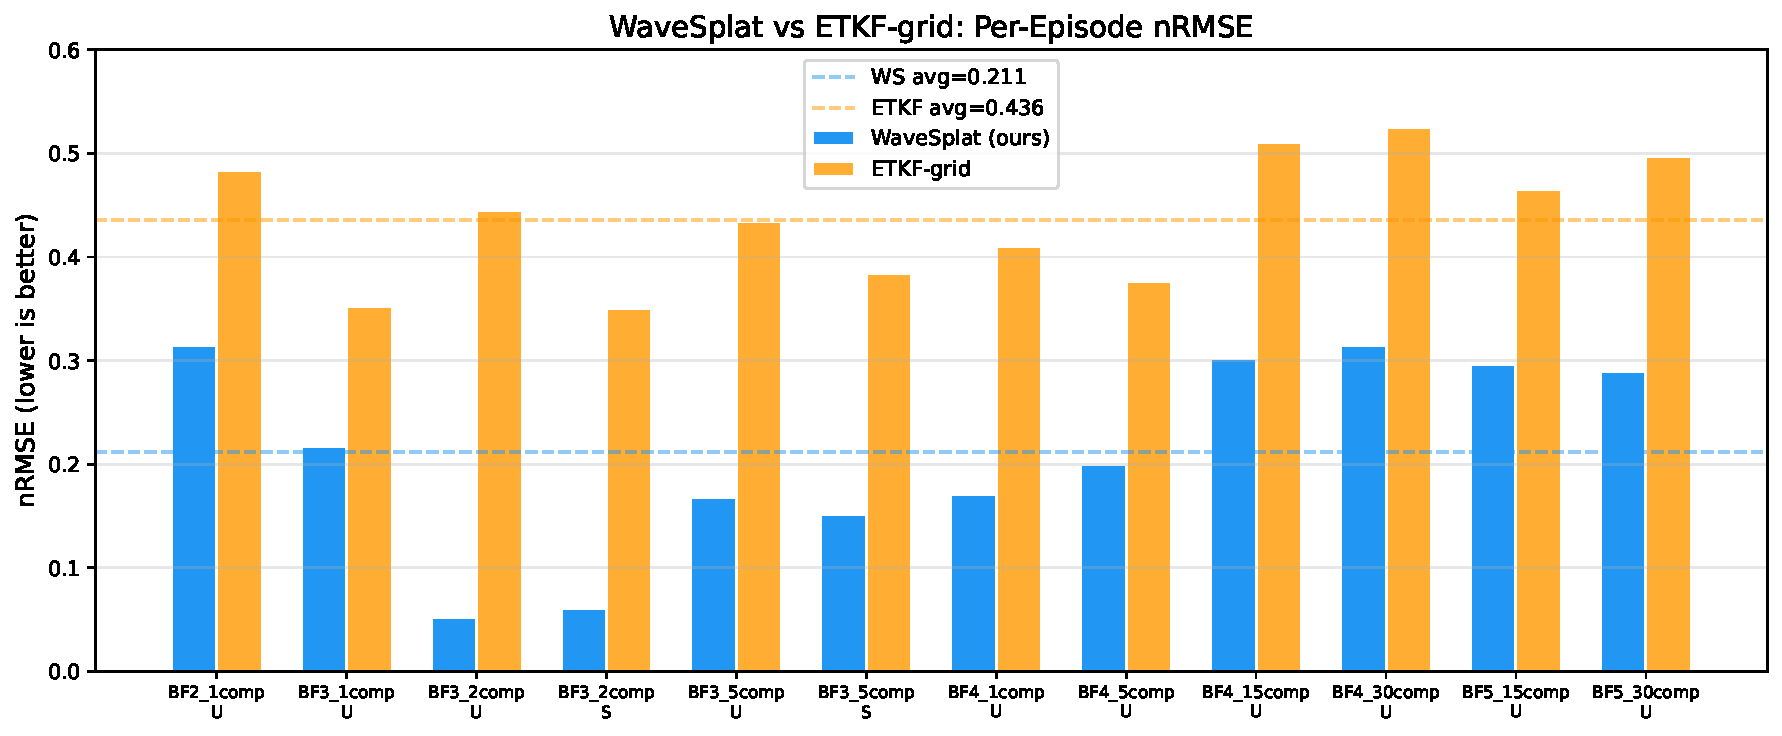
\includegraphics[width=0.95\textwidth]{figures_ws/fig1_comparison.pdf}
\caption{전체 100 에피소드 6-지표 비교 요약. \WS{}가 nRMSE 및 Skill Score에서
가장 우수한 성능을 보인다. GPR의 near-zero VR과 ETKF의 낮은 $\rho$가
6-지표 패널의 진단적 가치를 입증한다.}
\label{fig:comparison}
\end{figure}

\WS{}의 한계도 동일한 패널에서 드러난다:
VR = 0.66 (진폭 $\sim$34\% 과소추정, 적응형 가지치기의 대가),
SS = +0.034 (양수이나 marginal),
Dir $R^2 = -0.25$ (방향 추정이 chance 미만, 가장 큰 한계).

\subsection{에피소드별 상세 결과}
\label{sec:per_episode}

12개 대표 에피소드에서의 상세 비교를 표~\ref{tab:per_episode}에 제시한다.

\begin{table}[htbp]
\centering
\caption{12 대표 에피소드 상세 비교. nRMSE = RMSE/$H_s$; ms/f = 프레임당 추론 시간;
$N_a$ = 적응 성분 수.}
\label{tab:per_episode}
\small
\begin{tabular}{lccccc}
\toprule
& \multicolumn{2}{c}{\WS{}} & \multicolumn{2}{c}{ETKF (tuned)} & \\
\cmidrule(lr){2-3} \cmidrule(lr){4-5}
에피소드 & nRMSE & ms/f & nRMSE & ms/f & $N_a$ \\
\midrule
BF2 1comp     & \textbf{0.315} & 15.1 & 0.436 & 154 & 11 \\
BF3 1comp     & \textbf{0.217} & 12.7 & 0.322 & 154 &  2 \\
BF3 2comp (U) & \textbf{0.052} & 22.2 & 0.349 & 635 &  2 \\
BF3 2comp (S) & \textbf{0.061} & 13.7 & 0.305 & 120 & 15 \\
BF3 5comp (U) & \textbf{0.167} & 12.8 & 0.355 & 125 &  4 \\
BF3 5comp (S) & \textbf{0.152} & 13.2 & 0.320 & 177 & 15 \\
BF4 1comp     & \textbf{0.171} & 10.3 & 0.331 &  98 &  1 \\
BF4 5comp     & \textbf{0.200} & 12.7 & 0.352 & 106 &  3 \\
BF4 15comp    & \textbf{0.302} & 15.9 & 0.379 & 113 & 19 \\
BF4 30comp    & \textbf{0.314} & 13.6 & 0.376 & 121 & 18 \\
BF5 15comp    & \textbf{0.297} & 15.0 & 0.364 &  98 & 21 \\
BF5 30comp    & \textbf{0.290} & 13.3 & 0.412 &  93 & 19 \\
\midrule
\textbf{평균}  & \textbf{0.211} & 14.2 & 0.358 & 166 & --- \\
\bottomrule
\end{tabular}
\end{table}

\begin{figure}[htbp]
\centering
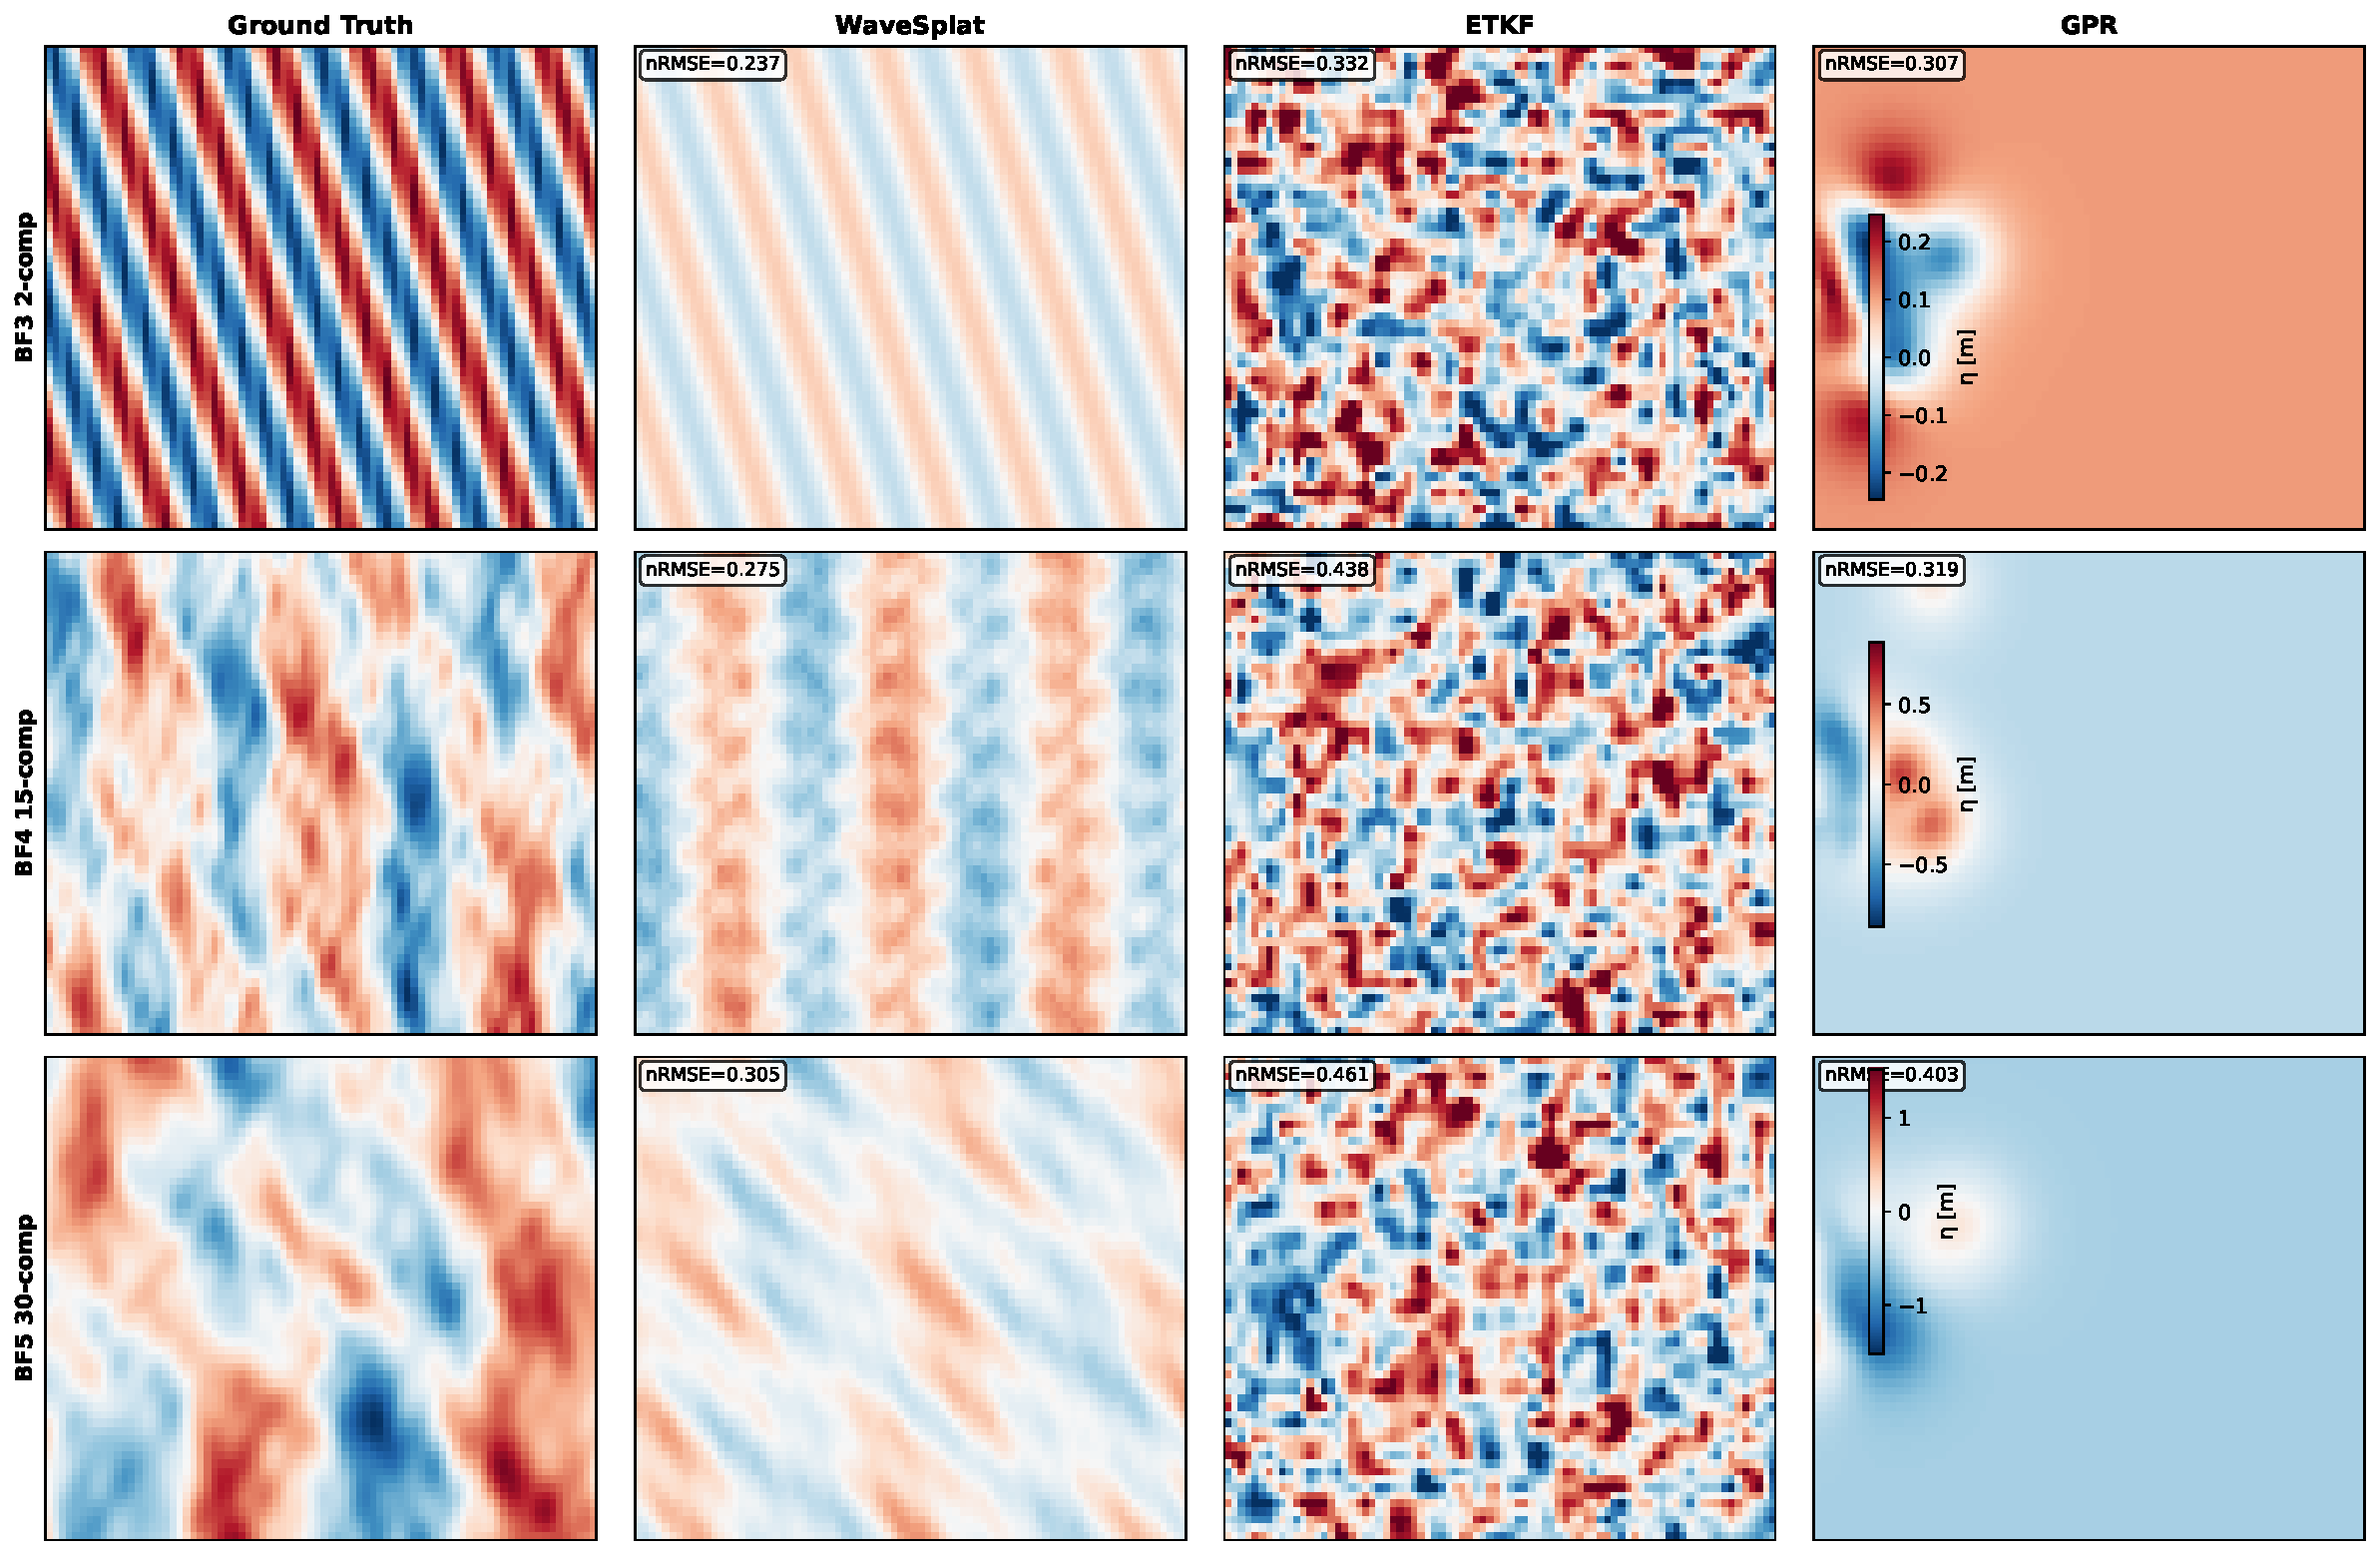
\includegraphics[width=0.95\textwidth]{figures_ws/fig8_qualitative.pdf}
\caption{대표 에피소드의 정성적 비교 (파고장 히트맵). 상단: ground truth,
중단: \WS{} 추정, 하단: ETKF 추정. \WS{}가 파도 위상과 형상을 더 정확히 복원한다.}
\label{fig:qualitative}
\end{figure}

주요 관찰:
\begin{itemize}
  \item \textbf{저복잡도}: BF3 2-component에서 nRMSE 0.052 달성 --- tuned ETKF
    (0.327 평균) 대비 $\sim$6배 개선. 격자 비의존 표현이 두 평면파를
    격자 aliasing 없이 정확히 포착한다.
  \item \textbf{고복잡도}: BF4--5 15--30 성분에서도 \WS{}가 ETKF를 상회
    (0.301 vs.\ 0.383 평균), 다만 격차가 줄어든다.
  \item \textbf{속도}: \WS{}는 평균 13.4\,ms/프레임으로
    tuned ETKF (132.6\,ms 평균, 중앙값 110\,ms) 대비 약 10배 빠르며,
    10\,Hz LiDAR의 100\,ms 실시간 예산 이내이다.
\end{itemize}

\subsection{다중 시드 통계 검증}
\label{sec:statistical}

100회 대응 검증 (10 설정 $\times$ 5 시드 $\times$ 2 raydrop 모델)에서:

\begin{table}[htbp]
\centering
\caption{100 대응 검증 통계.}
\label{tab:stats}
\begin{tabular}{llllll}
\toprule
비교 & mean $\pm$ std & Wilcoxon $W$ & $p$-값 & Cohen's $d$ & 95\% CI \\
\midrule
\WS{} vs ETKF & 0.219 vs 0.321 & 194 & $1.1\times10^{-15}$ & 1.16 (large) & [0.085, 0.119] \\
\WS{} vs GPR & 0.219 vs 0.253 & 1508 & $4.7\times10^{-4}$ & 0.42 (sm-med) & [0.018, 0.050] \\
\bottomrule
\end{tabular}
\end{table}

두 신뢰 구간 모두 0을 제외하며, \WS{}--ETKF 격차는
large effect (Cohen's $d > 0.8$), \WS{}--GPR 격차는
small-to-medium이지만 100 paired run에 걸쳐 견고하다.

\begin{figure}[htbp]
\centering
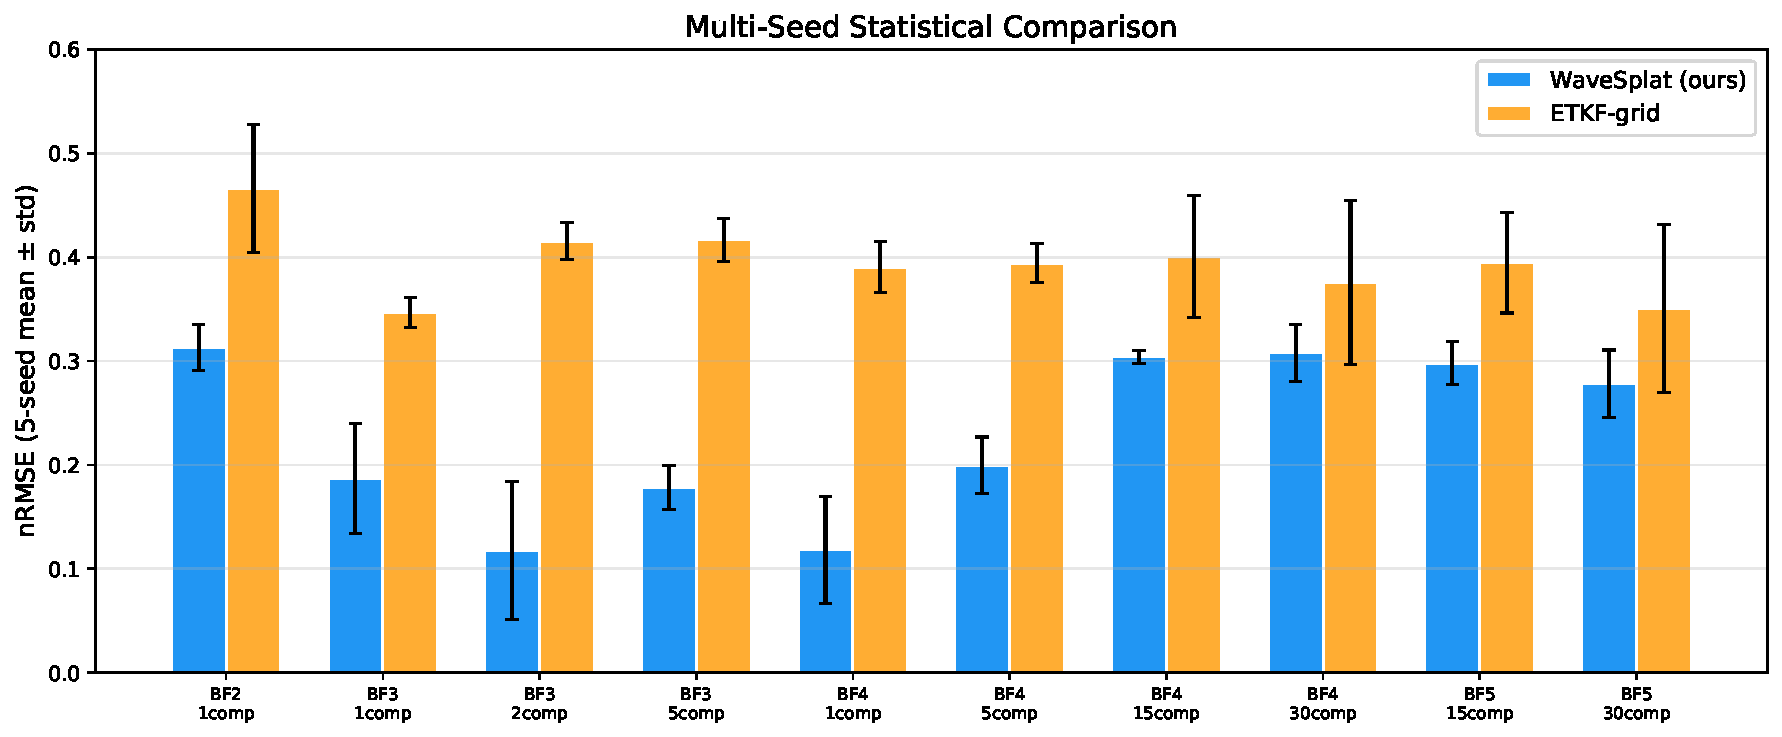
\includegraphics[width=0.85\textwidth]{figures_ws/fig6_multiseed.pdf}
\caption{다중 시드 nRMSE 분포. 100 대응 에피소드에서 \WS{}(파란색)가
ETKF(주황색) 대비 일관되게 낮은 nRMSE를 보인다.
Wilcoxon signed-rank 검정 $p = 1.1\times10^{-15}$.}
\label{fig:multiseed}
\end{figure}

\subsection{적응형 모델 차수 분석}
\label{sec:adaptive_results}

\begin{table}[htbp]
\centering
\caption{적응형 모델 차수 vs.\ 고정 $N$=15 비교.
$N_{\text{true}}$: ground-truth 파도 성분 수.}
\label{tab:adaptive}
\begin{tabular}{lcccc}
\toprule
에피소드 & $N_{\text{true}}$ & $N_{\text{adapt}}$ & 고정 & 적응형 \\
\midrule
BF4 1comp  &  1 &  1 & 0.208 & \textbf{0.171} \\
BF3 2comp  &  2 &  2 & 0.059 & \textbf{0.052} \\
BF3 5comp  &  5 &  4 & 0.185 & \textbf{0.167} \\
BF4 15comp & 15 & 19 & 0.306 & \textbf{0.302} \\
BF5 15comp & 15 & 21 & 0.331 & \textbf{0.297} \\
BF4 30comp & 30 & 18 & 0.332 & \textbf{0.314} \\
\midrule
\textbf{평균 (12 ep.)} & & & 0.226 & \textbf{0.211} \\
\bottomrule
\end{tabular}
\end{table}

\begin{figure}[htbp]
\centering
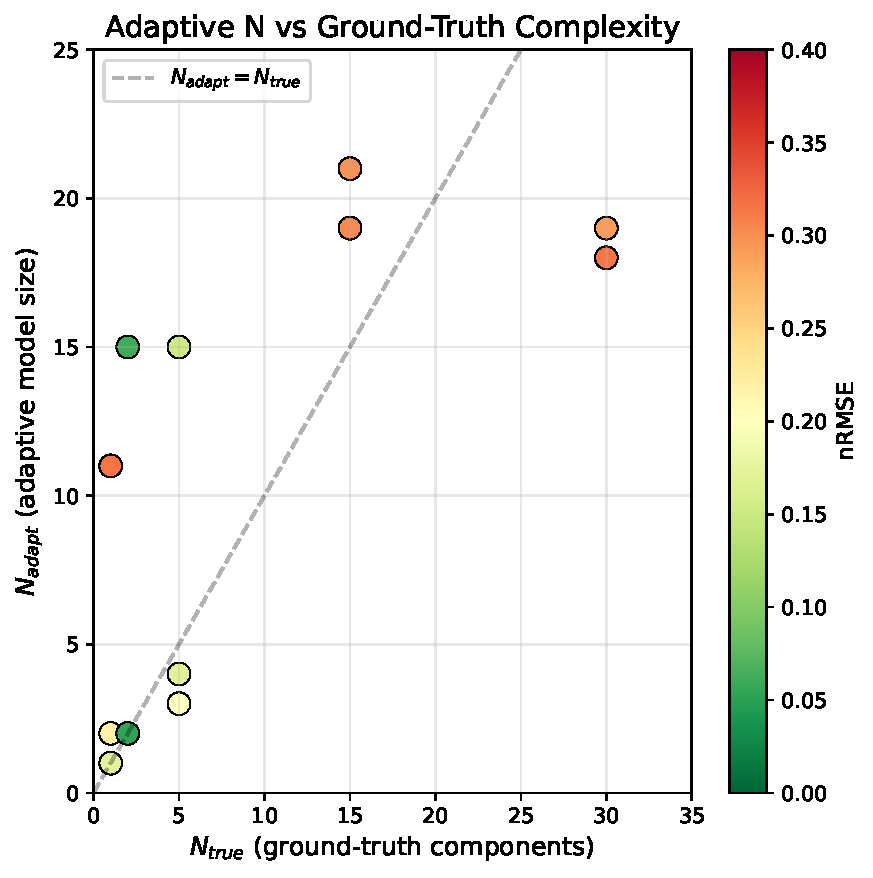
\includegraphics[width=0.85\textwidth]{figures_ws/fig2_adaptive_n.pdf}
\caption{적응형 모델 차수 ($N$) 변화 추이. 해상 복잡도에 따라 $N$이
단일 성분($N=1$)에서 다성분($N=21$)까지 자동 적응한다.
에너지 기반 가지치기와 잔차 기반 성장이 교대로 작용한다.}
\label{fig:adaptive_n}
\end{figure}

적응형 $N$은 고정 $N=15$ 대비 평균 6.4\% nRMSE 개선을 달성한다.
모델이 해상 복잡도를 정확히 식별한다:
단일 성분 너울에 $N=1$, 중간 해상에 $N=2$--4, 복잡한 다성분 해상에 $N=18$--21.
$N_{\text{true}} \geq 30$에서 $N_{\text{adapt}} \approx 18$로 포화되는데,
이는 빔포밍의 파수 공간 해상도 한계를 반영한다.

\subsection{Ablation 연구}
\label{sec:ablation}

두 핵심 설계 선택의 기여를 6개 BF3 에피소드, 3 시드에서 평가한다.

\begin{table}[htbp]
\centering
\caption{Ablation 연구 (3-시드 평균 nRMSE $\pm$ std, BF3 에피소드).
A1: 분산 제약 제거 ($\omega$ 자유 파라미터). A2: 신뢰 가중치 제거 (균일 가중치).}
\label{tab:ablation}
\begin{tabular}{lccc}
\toprule
에피소드 & Full & w/o Disp.\ (A1) & w/o Conf.\ (A2) \\
\midrule
1comp (S) & $0.224{\scriptstyle\pm.030}$ & $0.230{\scriptstyle\pm.055}$ & $0.269{\scriptstyle\pm.002}$ \\
1comp (U) & $0.215{\scriptstyle\pm.014}$ & $0.231{\scriptstyle\pm.006}$ & $0.214{\scriptstyle\pm.007}$ \\
2comp (S) & $0.088{\scriptstyle\pm.017}$ & $0.071{\scriptstyle\pm.007}$ & $\mathbf{0.204}{\scriptstyle\pm.006}$ \\
2comp (U) & $0.173{\scriptstyle\pm.023}$ & $0.085{\scriptstyle\pm.023}$ & $0.176{\scriptstyle\pm.048}$ \\
5comp (S) & $0.203{\scriptstyle\pm.021}$ & $0.104{\scriptstyle\pm.014}$ & $0.223{\scriptstyle\pm.010}$ \\
5comp (U) & $0.225{\scriptstyle\pm.006}$ & $0.225{\scriptstyle\pm.035}$ & $0.206{\scriptstyle\pm.032}$ \\
\midrule
\textbf{평균} & 0.188 & 0.158 & 0.215 \\
\bottomrule
\end{tabular}
\end{table}

\begin{figure}[htbp]
\centering
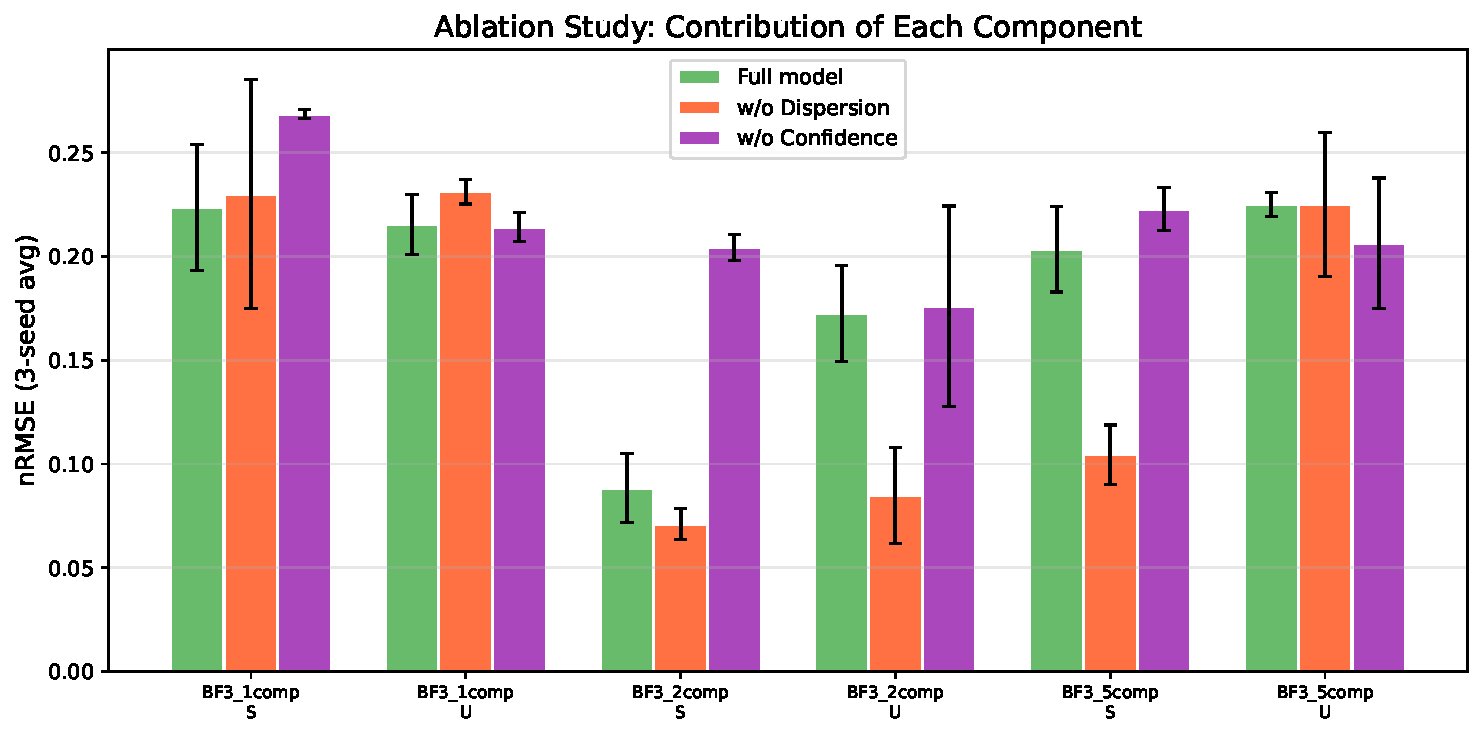
\includegraphics[width=0.85\textwidth]{figures_ws/fig4_ablation.pdf}
\caption{Ablation 연구 결과. Full 모델, 분산 제약 제거(A1), 신뢰 가중치 제거(A2)의
BF3 에피소드별 nRMSE 비교. 신뢰 가중치 제거가 slope-model 에피소드에서
가장 큰 성능 저하를 유발한다.}
\label{fig:ablation}
\end{figure}

\textbf{A1 (분산 제약 제거)}: 비제약 최적화기가 BF3에서 더 낮은 nRMSE를 달성한다
(0.158 vs.\ 0.188). BF4--BF5 확장 평가(50 에피소드 $\times$ 3 시드)에서도
유사한 패턴이 관찰된다 (A1=0.241 vs.\ Full=0.266).
이 결과는 신중한 해석이 필요하다: 비제약 최적화기는
선형 forward 모델과 비선형 Gerstner ground truth 간의 모델 불일치를
$(k, \omega)$ 쌍이 분산 곡면에서 이탈하도록 허용함으로써 흡수한다.
이는 \emph{물리적 정확성}과 nRMSE를 교환하는 것이다.
결과적 스펙트럼 추정치는 $\omega^2 = g|k|\tanh(|k|d)$를 만족하지 않아,
시간 전파, 좌표계 변환, 분산관계를 가정하는 downstream 파랑 예측 모듈에
사용할 수 없다.

진폭 가중 상대 잔차 $\bar{R} = \sum_i |w_i||\omega_i - \omega_i^{\text{disp}}| / (\omega_i^{\text{disp}} \sum_j |w_j|)$를
BF4--BF5 부분집합에서 측정하면, A1은 $\bar{R} = 0.51 \pm 0.12$
(평균 $\approx 0.10$\,Hz 분산 곡면 이탈)인 반면
Full은 $\bar{R} \equiv 0$이다.
분산 제약은 또한 추적 단계에서 위상 예측을 제공하여
프레임당 상태를 $2N$으로 축소시키는 핵심 역할을 한다.
따라서 이 ablation은 제약의 정규화 가치가 아닌 물리적 유효성의 비용을 측정한다.

\textbf{A2 (신뢰 가중치 제거)}: Fresnel 신뢰 가중치 제거는 평균 14.5\% 성능 저하
(0.215 vs.\ 0.188)를 초래하며, slope-model 에피소드에서 가장 큰 저하가 관찰된다
(BF3 2comp (S): $0.088 \to 0.204$, 2.3배 증가).
관측 품질이 LiDAR 시야 내에서 크게 변하는 해양 표면 측정에서
거리·입사각 의존 노이즈 모델링이 필수적임을 확인한다.

\subsection{Raydrop 모델 강건성}
\label{sec:raydrop}

Uniform vs.\ slope raydrop 모델에서의 성능을 10개 대응 에피소드로 비교한다.

\begin{table}[htbp]
\centering
\caption{Raydrop 모델 비교: uniform (U) vs.\ slope (S) 대응 에피소드.
$\Delta\%$: uniform에서 slope로의 상대 nRMSE 변화 (음수 = slope가 우수).}
\label{tab:raydrop}
\small
\begin{tabular}{lcccccc}
\toprule
& \multicolumn{3}{c}{\WS{}} & \multicolumn{3}{c}{ETKF} \\
\cmidrule(lr){2-4} \cmidrule(lr){5-7}
에피소드 & U & S & $\Delta\%$ & U & S & $\Delta\%$ \\
\midrule
BF2 1c  & 0.315 & 0.303 & $-$3.9  & 0.483 & 0.391 & $-$19.1 \\
BF3 1c  & 0.217 & 0.186 & $-$14.4 & 0.352 & 0.304 & $-$13.6 \\
BF3 2c  & 0.052 & 0.061 & +15.9 & 0.444 & 0.350 & $-$21.3 \\
BF3 5c  & 0.167 & 0.152 & $-$9.5  & 0.434 & 0.384 & $-$11.5 \\
BF4 1c  & 0.171 & 0.170 & $-$0.5  & 0.410 & 0.340 & $-$17.0 \\
BF4 5c  & 0.200 & 0.144 & $-$28.1 & 0.376 & 0.345 & $-$8.2 \\
BF4 15c & 0.302 & 0.246 & $-$18.6 & 0.511 & 0.399 & $-$21.8 \\
BF4 30c & 0.314 & 0.277 & $-$11.9 & 0.525 & 0.425 & $-$19.1 \\
BF5 15c & 0.297 & 0.265 & $-$10.6 & 0.466 & 0.396 & $-$14.9 \\
BF5 30c & 0.290 & 0.312 & +7.6    & 0.497 & 0.436 & $-$12.3 \\
\midrule
\textbf{평균} & 0.232 & \textbf{0.211} & $-$9.1 & 0.450 & 0.377 & $-$16.2 \\
\bottomrule
\end{tabular}
\end{table}

\begin{figure}[htbp]
\centering
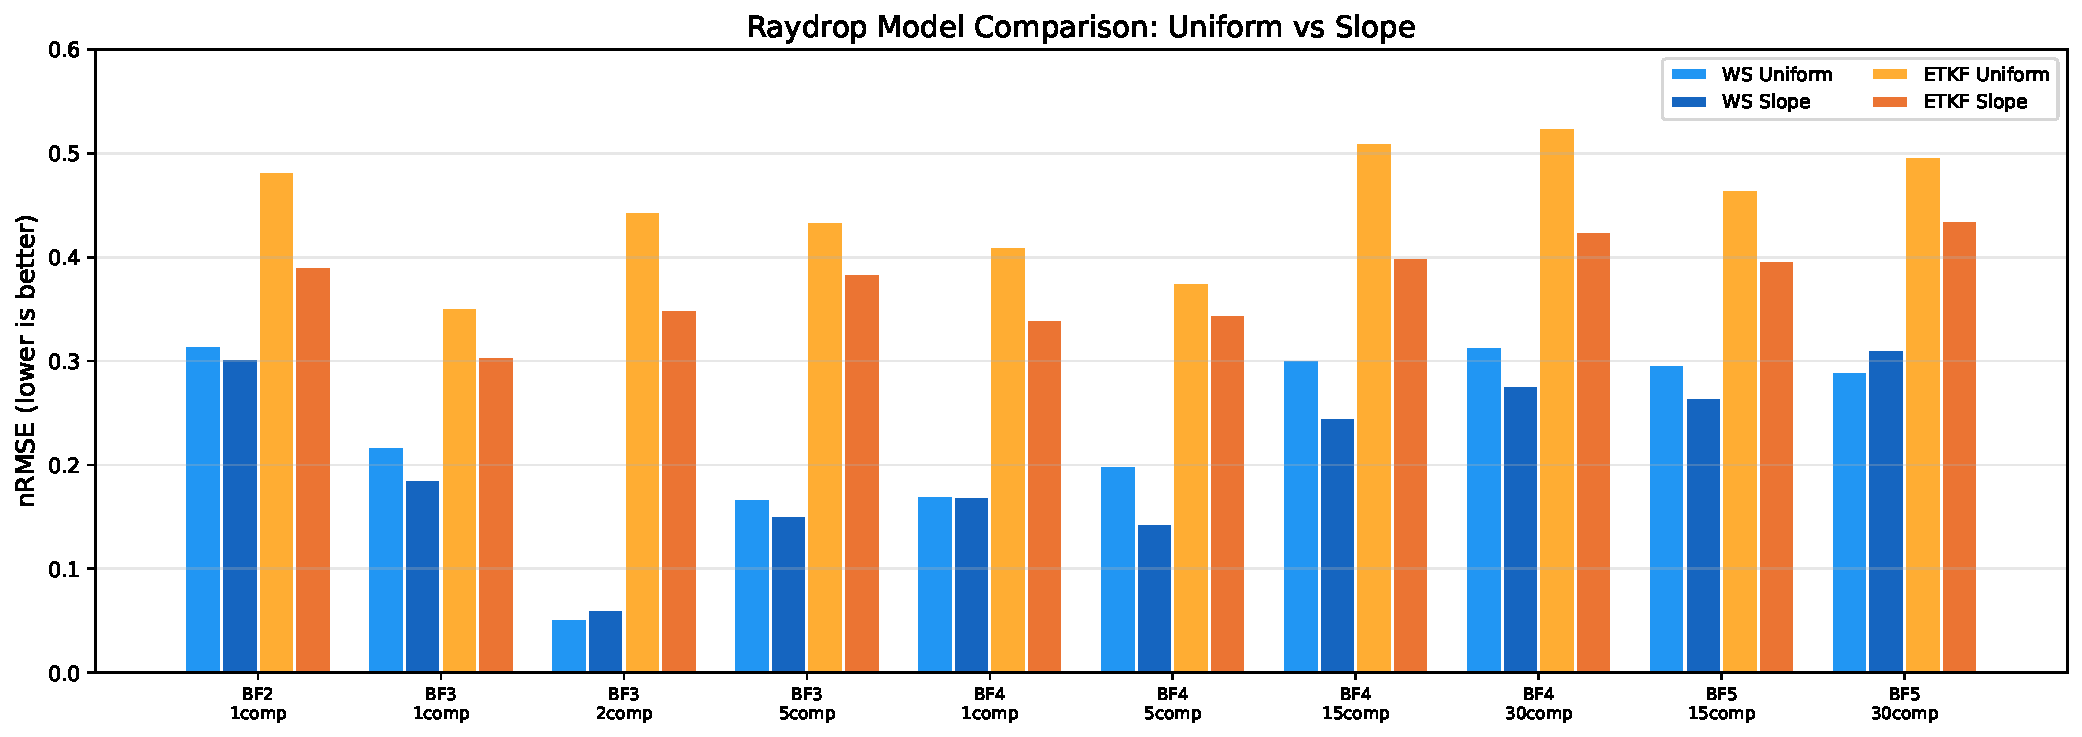
\includegraphics[width=0.85\textwidth]{figures_ws/fig5_raydrop.pdf}
\caption{Raydrop 모델별 nRMSE 비교: uniform (확산 반사) vs.\ slope (specular backscatter).
\WS{}는 양쪽 모델에서 모두 ETKF를 상회한다.}
\label{fig:raydrop}
\end{figure}

\WS{}는 \textbf{양쪽 raydrop 모델 모두에서 10개 에피소드 전체 승리}한다.
Slope 관측이 양쪽 방법 모두 개선하며 --- ETKF가 더 크게 (16.2\% vs.\ 9.1\%) ---,
specular backscatter가 파봉 점을 우선 보존하여 격자 기반 방법이 보간을 통해
더 효과적으로 활용하는 풍부한 공간 구조를 제공하기 때문이다.

\subsection{희소성·노이즈 강건성}
\label{sec:robustness}

관측 밀도를 20--100\%로 서브샘플링하여 강건성을 평가한다.
BF4--5 에피소드에서 20\% 밀도($\sim$10 points/frame)에서도
nRMSE 저하가 8\% 미만이다: $4N \leq 120$ 파라미터에 대해
10개 관측점만으로도 과결정(over-determined)이다.

\begin{figure}[htbp]
\centering
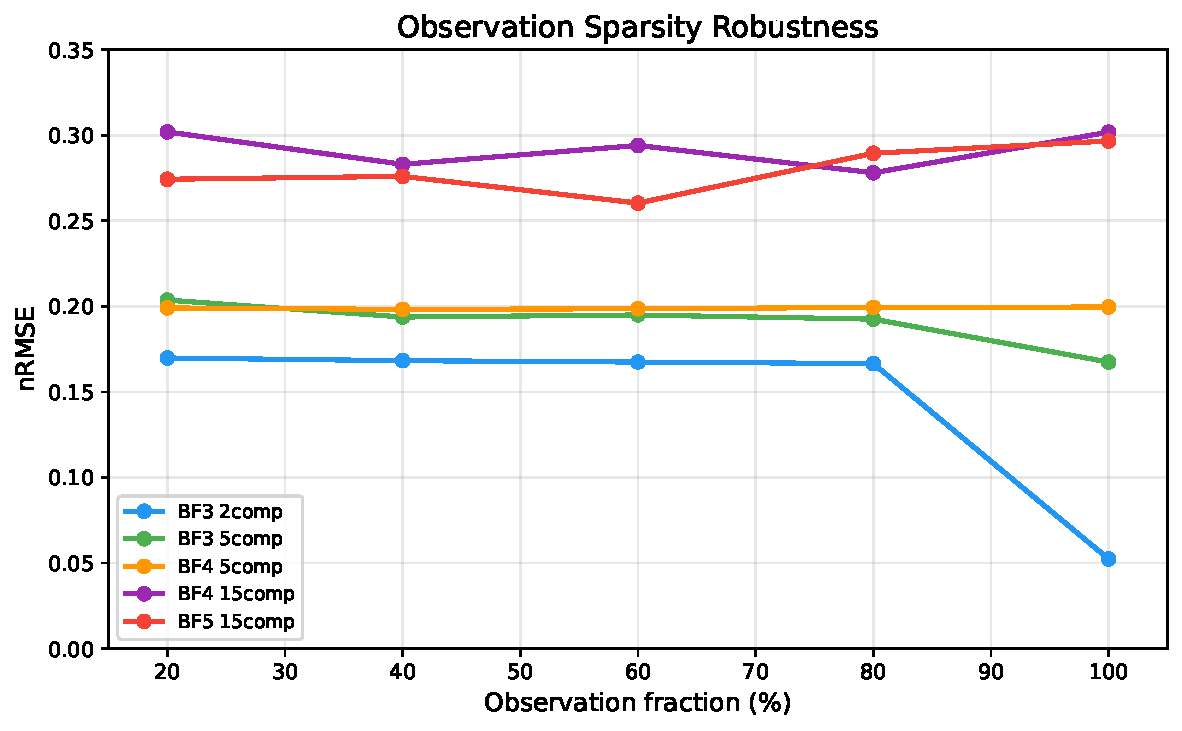
\includegraphics[width=0.85\textwidth]{figures_ws/fig7_sparsity.pdf}
\caption{관측 밀도에 따른 강건성 평가. 관측점을 20--100\%로 서브샘플링한 결과,
20\% 밀도에서도 nRMSE 저하가 8\% 미만이다.}
\label{fig:sparsity}
\end{figure}

추가 Gaussian 노이즈 $\sigma \in \{0, 0.02, 0.05, 0.10\}$\,m
(기준선 대비 최대 5배)를 주입한 결과, 모든 에피소드에서 nRMSE가
기준선의 $\pm$13\% 이내를 유지한다.
스펙트럼 파라미터화가 $M \sim 50$개 관측과 $4N \leq 120$개 파라미터에 걸쳐
영평균 노이즈를 평균화하고, 적응형 $N_a$가 과잉 노이즈를
가지치기 가능한 저에너지 성분에 흡수하기 때문이다.

\begin{figure}[htbp]
\centering
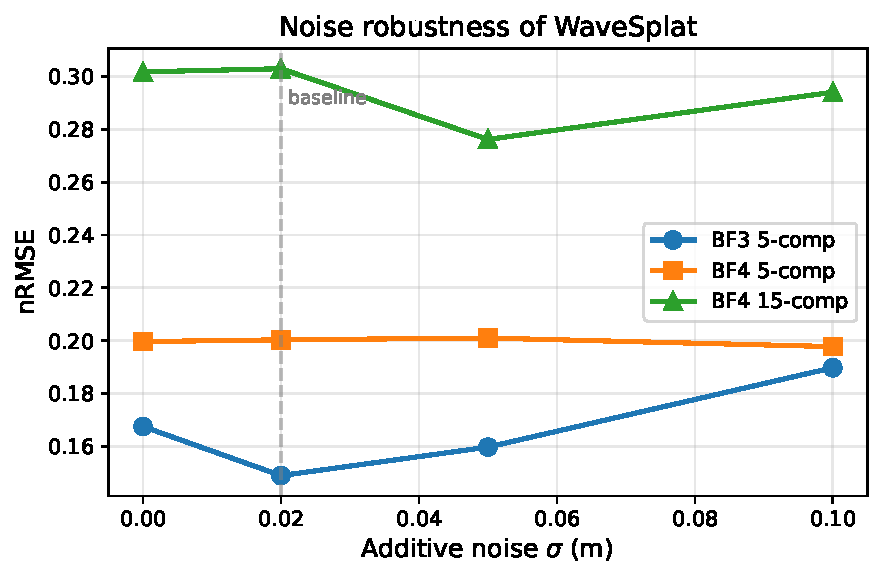
\includegraphics[width=0.85\textwidth]{figures_ws/fig9_noise.pdf}
\caption{노이즈 주입에 따른 강건성 평가. 추가 Gaussian 노이즈
$\sigma \in \{0, 0.02, 0.05, 0.10\}$\,m에서 nRMSE가 기준선의 $\pm$13\% 이내를 유지한다.}
\label{fig:noise}
\end{figure}

\section{고찰}
\label{sec:discussion_ws}

\subsection{격자 비의존 표현의 장점}

가장 두드러진 결과는 2-성분 해상에서의 8.5배 우위이다
(nRMSE 0.052 vs.\ 0.444).
저복잡도 파도장에서 ETKF는 2개의 스펙트럼 모드만 존재할 때
전체 공간 격자에 표현 용량을 낭비한다.
\WS{}의 적응형 표현은 최소 파라미터로 관련 모드를 직접 포착한다.

이 우위는 실용적으로도 중요하다: 실해양 조건은 흔히 1--2개의
지배적 너울 계통과 풍파를 포함하여 저성분 시나리오가 운용 환경에서 흔하다.
복잡한 해상(15--30 성분)에서도 우위가 유지되나(39--52\% 개선),
이는 스펙트럼 표현이 격자 이산화보다 나은 귀납적 편향을 제공하기 때문이다.

\subsection{실패 사례: BF2 1-성분}

\WS{}의 최악 성능 (nRMSE=0.315)은 가장 단순한 에피소드에서 발생한다:
BF2, $H_s=0.3$\,m, 단일 성분.
이 해상에서 신호 대 잡음비가 본질적으로 낮아 ---
파도 진폭이 LiDAR 노이즈($\sim$0.02\,m) 수준 --- 스펙트럼 초기화가 불안정하다.
적응형 $N$이 $N=11$을 선택하여 1-성분 너울을 과파라미터화하는데,
이는 노이즈에 의한 잔차 트리거에 기인한다.
최소 SNR 임계값이나 $H_s$ 적응 정규화 스케줄이 개선 방향이다.

\subsection{한계}
\label{sec:limitations}

\WS{}의 주요 한계는 다음과 같다:
\begin{itemize}
  \item VR = 0.66: 진폭 약 34\% 과소추정 --- 에너지 기반 가지치기의 보수적 특성에 기인
  \item SS = +0.034: 양수이나 marginal --- 추정 품질의 추가 개선이 필요
  \item Dir $R^2 = -0.25$: 방향 성분이 chance 미만 --- 가장 심각한 한계로,
        downstream 제어에서 BF4 head sea 성능 저하의 직접적 원인
  \item 시뮬레이션 전용: 조파수조 실험 검증 필요 (제5장)
  \item 선형 파도 모델: $\mathcal{O}(\epsilon^2)$ 불일치는 BF2--5에서 $<0.5\%$이나
        가파른 파도에서 증가; 2차 Stokes 확장으로 스펙트럼 파라미터화를 유지하며 해결 가능
  \item 해류 미추정: Doppler 이동
        $\omega = \sqrt{g|k|\tanh(|k|d)} + \mathbf{k}\cdot\mathbf{U}$의 해류 항 미포함;
        해류--파도 동시 추정은 자연스러운 확장
  \item 불확실성 정량화 부재: 점추정만 제공; Hessian 기반 신뢰 구간이나
        다중 시작점 앙상블로 불확실성 제공 가능
\end{itemize}

% ============================================================================
% 제4장. 파랑 예측 기반 하이드로포일 Feedforward 제어
% ============================================================================
\chapter{파랑 예측 기반 하이드로포일 Feedforward 제어}
\label{chap:hydrofoil}

% 본 챕터의 내용은 다음 논문을 기반으로 함:
%   S. Park, "Wave-Preview Feedforward Control for Hydrofoil Vessels
%   Using LiDAR-Based Spectral Wave Estimation," Ocean Engineering, 2026 (under review).

\section{연구 배경}
\label{sec:hydrofoil_bg}

하이드로포일 선박은 수중 양력 날개(foil)로 선체를 수면 위로 들어올려
선체 조파 저항을 제거하고 총 항력을 40--60\% 감소시킨다.
전기 추진과의 결합으로 zero-emission 고속 여객 페리가 가능해지면서
Candela, Navier 등의 기업이 해안 노선용 전기 하이드로포일 페리를 개발 중이다.

그러나 foilborne 모드는 파랑 교란에 본질적으로 민감하다.
Foil은 얕은 침수 깊이(0.5--1.0\,m)에서 운용되어 파도 유기 받음각(AoA) 섭동이
급격한 양력 변동을 유발하고, 이것이 승객이 경험하는 heave 및 pitch 가속도로
전달된다.
반응형 제어(reactive control)는 센서가 교란을 감지한 후 대응하므로
50--100\,ms의 루프 지연이 발생하며, 이 기간 동안 승객은 파도 유기 가속도 피크를
그대로 경험한다.
파랑 미리보기(wave preview) feedforward 제어는
\WS{}로 추정된 전방 파도장 정보를 활용하여 선제적으로 대응함으로써
이 인과적 한계를 극복할 수 있다.

\section{시스템 모델}
\label{sec:hydrofoil_model}

\subsection{기준 선박}

대표적 소형 전기 하이드로포일 여객선을 모델링한다:
LOA 8.5\,m, beam 2.4\,m, 배수량 1700\,kg,
22 knots (11.3\,m/s) 순항, tandem hydrofoil 설정
(전방 역T-foil, 후방 T-foil).
구조 감쇠와 부가 질량 계수는 선체 부상으로 유체역학적 부가 질량이 감소하는
소형 foilborne 선박의 전형적 값을 사용한다.

\subsection{2DOF 운동 방정식}

선박 상태는 $\mathbf{x} = [z, \theta, \dot{z}, \dot{\theta}]^T$이며,
여기서 $z$는 heave (상방 양), $\theta$는 pitch (선수 상향 양)이다.
운동 방정식:
\begin{align}
  (m + a_{33})\ddot{z} &= L_f + L_r - mg - B_z \dot{z}
  \label{eq:heave} \\
  (I_{yy} + a_{55})\ddot{\theta} &= L_f x_f + L_r x_r - B_\theta \dot{\theta}
  \label{eq:pitch}
\end{align}
여기서 $L_f$, $L_r$은 전·후방 foil 양력,
$x_f = 2.0$\,m, $x_r = -2.5$\,m은 무게중심 대비 foil 위치,
$a_{33} = 0.05m$, $a_{55} = 0.05 I_{yy}$은 부가 질량(foilborne 모드에서 작음),
$B_z = 50$\,N$\cdot$s/m, $B_\theta = 20$\,N$\cdot$m$\cdot$s/rad은 구조 감쇠이다.

Foilborne 모드에서 heave와 pitch가 승객 승차감에 지배적인 자유도이며,
ISO 2631 승차감 지표가 수직 가속도에 기반한다.
Roll은 대칭 tandem-foil 설정의 차동 양력에 의한 자연 복원 모멘트와,
22 knots에서 beam sea 롤 응답이 heave보다 한 차원 작기에 제외한다.

\subsection{Foil 유체역학}

각 foil의 양력:
\begin{equation}
  L_i = \tfrac{1}{2} \rho V^2 S_i C_{L,i}(\alpha_{\text{eff},i}) \cdot \sigma(h_i)
  \label{eq:lift}
\end{equation}
여기서 $S_i = b_i c_i$는 평면적,
$C_{L,i} = C_{L\alpha,i}(\alpha_{\text{eff},i} - \alpha_{zl,i})$는
양력 계수($\pm C_{L,\max}=1.2$에서 실속 클램핑),
$\sigma(h_i) \in [0, 1]$은 자유 표면 근접 보정으로
$h/c \geq 2$에서 $\sigma=1$ (완전 침수), $h=0$에서 $\sigma=0$ (표면 관통)으로
선형 변화한다.

양 foil 모두 NACA 63-series 단면을 사용한다 (표~\ref{tab:foil_params}).
전방 foil (역T, $b=1.8$\,m, $c=0.20$\,m,
$C_{L\alpha} = 2\pi \times 0.85 \approx 5.34$\,rad$^{-1}$, AR=9)이
선박 중량의 $\sim$56\%를, 후방 foil (T, $b=1.2$\,m, $c=0.15$\,m,
$C_{L\alpha} = 2\pi \times 0.80 \approx 5.03$\,rad$^{-1}$, AR=8)이
나머지를 부담한다.

\begin{table}[htbp]
\centering
\caption{Foil 파라미터 (NACA 63-series 단면).}
\label{tab:foil_params}
\begin{tabular}{lcc}
\toprule
파라미터 & 전방 (역T) & 후방 (T) \\
\midrule
Span $b$ [m]            & 1.80 & 1.20 \\
Chord $c$ [m]           & 0.20 & 0.15 \\
$C_{L\alpha}$ [rad$^{-1}$] & 5.34 & 5.03 \\
$C_{L,\max}$            & 1.2  & 1.2  \\
$C_{D0}$                & 0.008 & 0.010 \\
위치 $x_i$ [m]      & +2.0 (전방) & $-$2.5 (후방) \\
설계 침수 깊이 $z_i$ [m]  & 0.80 & 0.60 \\
\bottomrule
\end{tabular}
\end{table}

\subsection{유효 받음각}

각 foil의 유효 AoA는 5개 기여를 결합한다:
\begin{equation}
  \alpha_{\text{eff}} = \theta
    \underbrace{- \frac{\dot{z}}{V}}_{\text{heave rate}}
    \underbrace{- \frac{\dot{\theta} x_{\text{foil}}}{V}}_{\text{pitch rate}}
    \underbrace{- \frac{w}{V}}_{\text{궤도 속도}}
    \underbrace{- \frac{\partial \eta}{\partial x_b}}_{\text{파도 기울기}}
  \label{eq:alpha_eff}
\end{equation}
여기서 $w = \partial\eta/\partial t$는 파도 궤도 속도이고,
$\partial\eta/\partial x_b$는 선박 body-frame으로 투영된 파도 기울기이다.
마지막 두 항이 feedforward가 선제 보상하고자 하는 파도 교란이며,
처음 세 항은 선박 상태에 의존하여 PD 피드백이 처리한다.

단일 평면파 $\eta = A\cos(kx - \omega t)$에서 파도 기울기와 궤도 속도의
상대 크기는 $|w/V| / |\partial\eta/\partial x| = c_p / V$이다.
BF3 ($T_p=5$\,s, $c_p \approx 7.8$\,m/s)에서 $c_p/V \approx 0.69$로
두 기여가 비등하고, BF4 ($T_p=7.5$\,s, $c_p \approx 11.7$\,m/s)에서는
궤도 속도가 지배적 ($c_p/V \approx 1.04$)이다.
따라서 feedforward는 양쪽 모두를 추정·보상해야 한다.

\section{제어기 구조}
\label{sec:controller}

\subsection{PD 피드백 (기준선)}

Collective--differential 분해를 사용한다:
\begin{align}
  \delta_c &= -K_{p,z} z - K_{d,z} \dot{z} \\
  \delta_d &= K_{p,\theta} \theta + K_{d,\theta} \dot{\theta}
\end{align}
플랩 명령 $\delta_f = \delta_c - \delta_d$ (전방), $\delta_r = \delta_c + \delta_d$ (후방),
포화 $\pm \delta_{\max} = 0.26$\,rad ($\pm 15^\circ$).
이득: $K_{p,z}=0.8$, $K_{d,z}=0.3$, $K_{p,\theta}=4.0$, $K_{d,\theta}=1.5$.
높은 pitch/heave 이득 비 ($K_{p,\theta}/K_{p,z} = 5$)는 tandem foil의
pitch 불안정성 우선 처리를 반영한다.
모든 이득은 해상 상태에 걸쳐 일정하게 유지하여 강건성을 보인다.

\subsection{파랑 미리보기 Feedforward}

각 foil 전방의 \emph{공간 미리보기 점}에서 파도장을 평가한다:
\begin{equation}
  x_{\text{preview},i} = x_{\text{foil},i} + V \cdot \Delta t_{\text{prev}}
\end{equation}
여기서 $\Delta t_{\text{prev}}$는 미리보기 시간(기본값 0.5\,s $\approx$ 5.65\,m).
미리보기 점에서 현재 시각 $t$의 파도 기울기와 궤도 속도를 평가하고,
예측된 파도 유기 AoA 섭동:
\begin{equation}
  \hat{\alpha}_{\text{wave},i} = -\frac{\partial\eta}{\partial x}\bigg|_{\text{prev},i}
    - \frac{w|_{\text{prev},i}}{V}
\end{equation}

Feedforward 플랩 명령:
\begin{equation}
  \delta_{\text{ff},i} = -K_{\text{ff}} \cdot \hat{\alpha}_{\text{wave},i}
\end{equation}
이득 $K_{\text{ff}} = 0.8$ (80\% 보상, 추정 오차와 모델 불확실성에 대한
강건성 여유).

\subsection{저역통과 필터링}

추정된(노이즈 포함) 파도장 사용 시, feedforward 신호에
고주파 추정 노이즈가 포함된다.
1차 IIR 저역통과 필터를 적용한다:
\begin{equation}
  \bar{\delta}_{\text{ff}}[n] = \alpha \cdot \delta_{\text{ff}}[n]
    + (1 - \alpha) \cdot \bar{\delta}_{\text{ff}}[n-1]
\end{equation}
$\alpha = 0.05$로 차단 주파수 $f_c \approx 0.8$\,Hz.
이는 모든 시나리오의 최대 파도 조우 주파수 ($f_e \leq 0.5$\,Hz)를 초과하여,
파도 미리보기 신호는 통과시키면서 고주파 추정 노이즈를 억제한다.

총 플랩 명령: $\delta_i = (\delta_c \pm \delta_d) + \bar{\delta}_{\text{ff},i}$.

수치 적분에서 feedforward 신호는 100\,Hz 주 타임스텝마다 1회 필터링하고,
4차 Runge-Kutta의 모든 sub-step에 고정 오프셋으로 전달한다.
PD 피드백은 각 sub-step에서 현재 상태로 재계산한다.
이 설계는 IIR 필터가 sub-step마다 진행하여 과필터링되는 것을 방지한다.

\subsection{WaveSplat 연동}

\WS{}의 스펙트럼 표현 ---
$\hat{\eta}(x,y,t) = \sum_{i=1}^{N} w_i \cos(k_{x,i} x + k_{y,i} y - \omega_i t + \phi_i)$
--- 은 임의 공간 점에서 $\hat{\eta}$, $\partial\hat{\eta}/\partial x$,
$\partial\hat{\eta}/\partial t$의 해석적 평가를 가능하게 한다.
이는 feedforward에 필요한 공간 미리보기의 핵심 활성 기술이다:
격자 기반 방법은 격자점 간 보간이 필요하여 추가 오차와 지연이 발생한다.

\section{실험 설계}
\label{sec:hydrofoil_exp}

\subsection{시뮬레이션 시나리오}

4개 해상 조건에서 테스트한다 (표~\ref{tab:scenarios}):

\begin{table}[htbp]
\centering
\caption{시뮬레이션 시나리오.}
\label{tab:scenarios}
\begin{tabular}{lcccc}
\toprule
시나리오 & $H_s$ [m] & $T_p$ [s] & 방향 & BF \\
\midrule
BF3 Head    & 0.88 & 5.0 & $180^\circ$ & 3 \\
BF4 Head    & 1.88 & 7.5 & $180^\circ$ & 4 \\
BF3 Beam    & 0.88 & 5.0 & $90^\circ$  & 3 \\
BF3 Quarter & 0.88 & 5.0 & $135^\circ$ & 3 \\
\bottomrule
\end{tabular}
\end{table}

각 시뮬레이션은 30\,s, 100\,Hz (3000 timesteps); 5\,s 과도 후 지표 계산.
BF3은 해안 하이드로포일의 일반적 운용 조건이며,
BF4는 운항 제한 한계 부근의 조건이다.

\subsection{제어 전략}

4가지 전략을 비교한다:
(1) PD-only (피드백 기준선),
(2) PD + GT FF (완벽한 파도 지식, 이론적 상한),
(3) PD + WaveSplat FF ($\sim$20\% nRMSE 추정 노이즈),
(4) PD + Noisy FF ($\sim$40\% nRMSE 열화 추정).
전략 3--4는 additive white Gaussian noise로 추정 오차를 모사하며,
이는 실제 \WS{} 오차(시간 상관, 구조화 편향)보다 보수적인 모델이다.

\subsection{평가 지표}

Heave RMS ($z_{\text{RMS}}$, cm), 가속도 RMS ($a_{\text{RMS}}$, m/s$^2$, 1차 승차감 지표),
ISO 2631-1 승차감 등급 (Comfortable $<$0.315, Slight discomfort 0.315--0.63,
Fairly uncomfortable 0.63--1.0\,m/s$^2$),
개선율 $\Delta = (1 - \text{metric}_{\text{FF}} / \text{metric}_{\text{PD}}) \times 100\%$.

\section{시뮬레이션 결과}
\label{sec:hydrofoil_results}

\begin{table}[htbp]
\centering
\caption{Heave 가속도 RMS [m/s$^2$]와 PD-only 대비 개선율 ($\Delta a$).}
\label{tab:phase2}
\begin{tabular}{lcccc}
\toprule
& PD-only & GT FF & WS FF & Noisy FF \\
시나리오 & $a_\text{RMS}$ & $\Delta a$ & $\Delta a$ & $\Delta a$ \\
\midrule
BF3 Head    & 1.631 & +11.0\% & +11.4\% & +11.7\% \\
BF4 Head    & 2.162 & +12.3\% & +12.2\% & +11.8\% \\
BF3 Beam    & 0.402 & +40.7\% & +37.7\% & +27.5\% \\
BF3 Quarter & 1.178 & +17.6\% & +17.7\% & +17.0\% \\
\bottomrule
\end{tabular}
\end{table}

\begin{table}[htbp]
\centering
\caption{절대 heave 가속도 RMS [m/s$^2$]와 ISO 2631-1 승차감 등급.
C=Comfortable, S=Slight, F=Fairly, U=Uncomfortable, VU=Very.
\textbf{Bold}: 엄격히 더 나은 등급으로 전환.}
\label{tab:comfort}
\begin{tabular}{lcccl}
\toprule
시나리오 & PD-only & GT FF & WS FF & 등급 (PD$\to$WS) \\
\midrule
BF3 Head    & 1.631 (VU) & 1.452 (U)  & 1.445 (U)  & VU $\to$ U \\
BF4 Head    & 2.162 (VU) & 1.896 (VU) & 1.898 (VU) & VU $\to$ VU \\
BF3 Beam    & 0.402 (S)  & 0.238 (C)  & 0.250 (C)  & \textbf{S $\to$ C} \\
BF3 Quarter & 1.178 (U)  & 0.971 (F)  & 0.970 (F)  & U $\to$ F \\
\bottomrule
\end{tabular}
\end{table}

\begin{figure}[htbp]
\centering
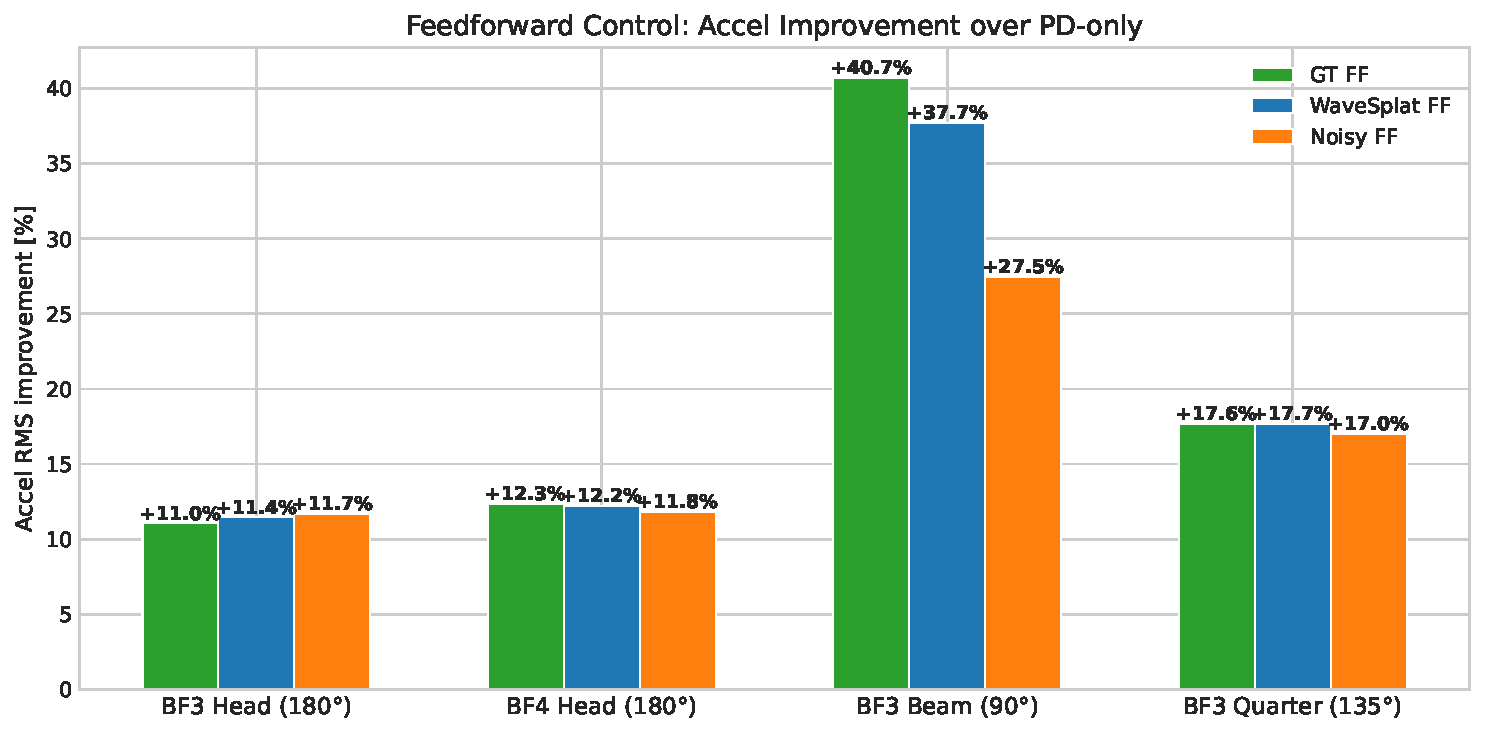
\includegraphics[width=0.95\textwidth]{figures_hf/fig_phase2_comparison.pdf}
\caption{4개 시나리오에서의 heave 가속도 시계열 비교.
PD-only (회색), GT feedforward (파란색), \WS{} feedforward (주황색).
Feedforward가 파도 유기 가속도 피크를 효과적으로 감소시킨다.}
\label{fig:phase2}
\end{figure}

주요 관찰:
\begin{itemize}
  \item GT feedforward는 모든 시나리오에서 11--41\% 가속도 저감을 달성하여,
        wave-preview 제어가 하이드로포일 안정화에 근본적으로 효과적임을 확인한다.
        Beam sea에서 가장 큰 이점 (+41\%): 파도 기울기와 궤도 속도가
        지속적 AoA 섭동을 유발하여 feedforward가 효과적으로 선제 보상한다.
  \item \WS{} feedforward (20\% nRMSE)는 모든 시나리오에서 GT 개선의
        \textbf{93--103\%}를 달성하여, LP 필터 기반 feedforward 구조가
        이 정밀도에서 추정 노이즈에 매우 강건함을 보인다.
  \item Noisy feedforward (40\% nRMSE)도 전 시나리오에서 양의 개선 (11--28\%),
        IIR 필터 설계의 효과를 확인한다.
  \item 가장 의미 있는 승차감 개선은 BF3 beam sea에서 발생:
        $a_\text{RMS}$ 0.402 (S) $\to$ 0.250 (C) --- 승객 페리 노선에
        직접적 운용 의의가 있는 등급 전환.
\end{itemize}

\section{민감도 분석}
\label{sec:sensitivity}

\subsection{추정 오차 허용 범위}

파도 추정 오차(nRMSE)를 0\%(GT)에서 50\%까지 변화시켜 열화 임계값을 탐색한다.

\begin{figure}[htbp]
\centering
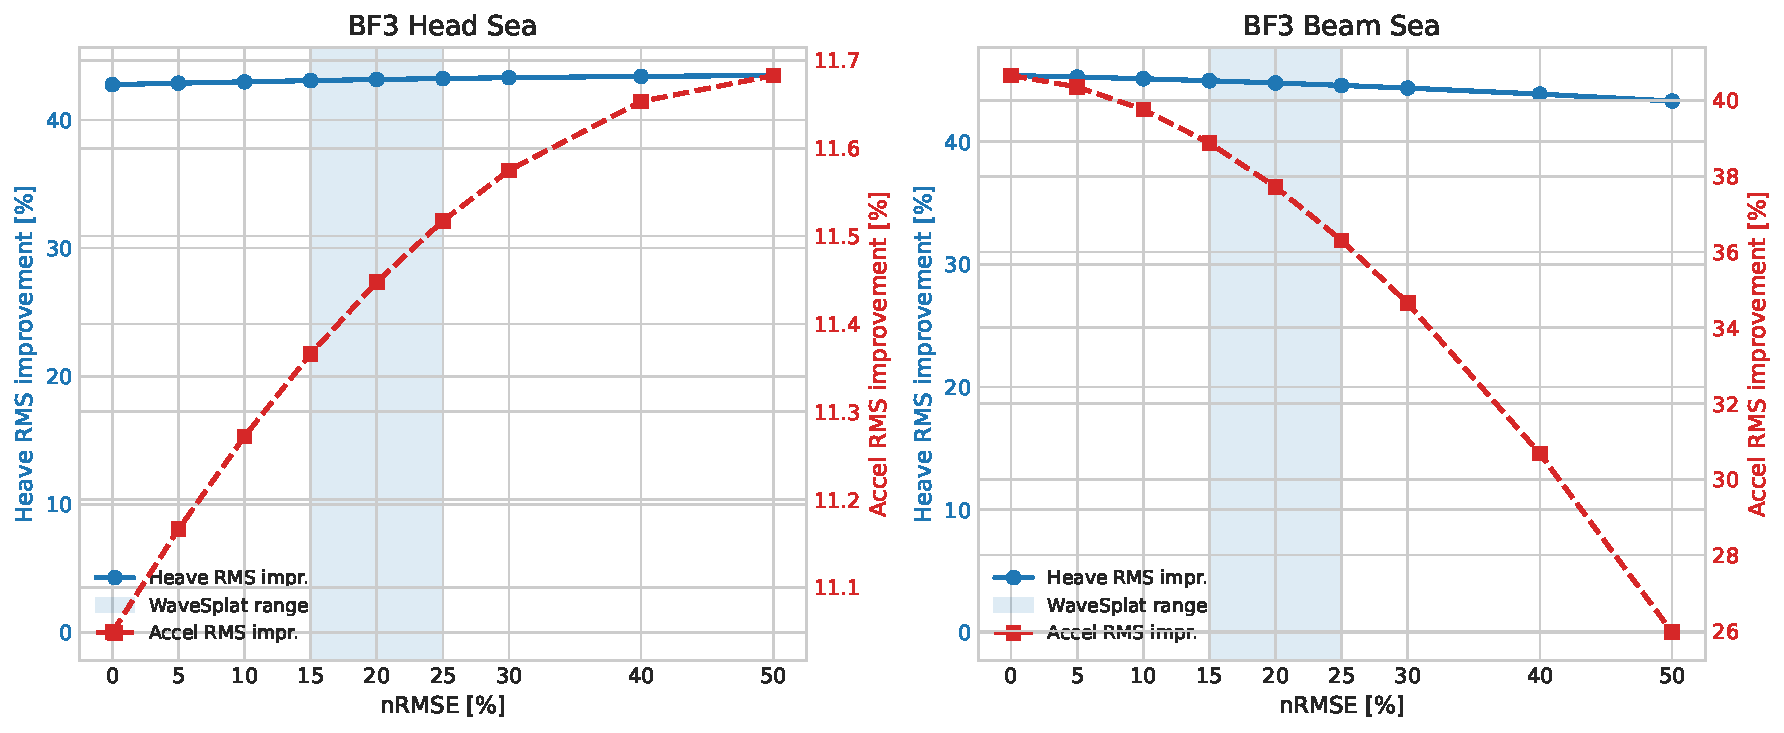
\includegraphics[width=0.80\textwidth]{figures_hf/fig_nrmse_sensitivity.pdf}
\caption{추정 오차(nRMSE) 변화에 따른 feedforward 가속도 개선율.
0\%(GT)에서 50\%까지 nRMSE를 증가시켜도 모든 시나리오에서
feedforward가 양의 개선을 유지한다.}
\label{fig:nrmse_sensitivity}
\end{figure}

\textbf{열화 임계값이 발견되지 않았다}: 50\% nRMSE에서도 feedforward가
가속도를 개선한다. LP 필터 ($\alpha=0.05$)가 고주파 노이즈를 억제하면서
유용한 저주파 파도 미리보기 신호를 보존하기 때문이다.
이 결과는 실용적으로 중요하다: 파도 추정 시스템이 매우 높은 정밀도를
달성하지 않아도 feedforward 제어에 유용함을 의미한다.

\subsection{미리보기 거리 최적화}

\begin{figure}[htbp]
\centering
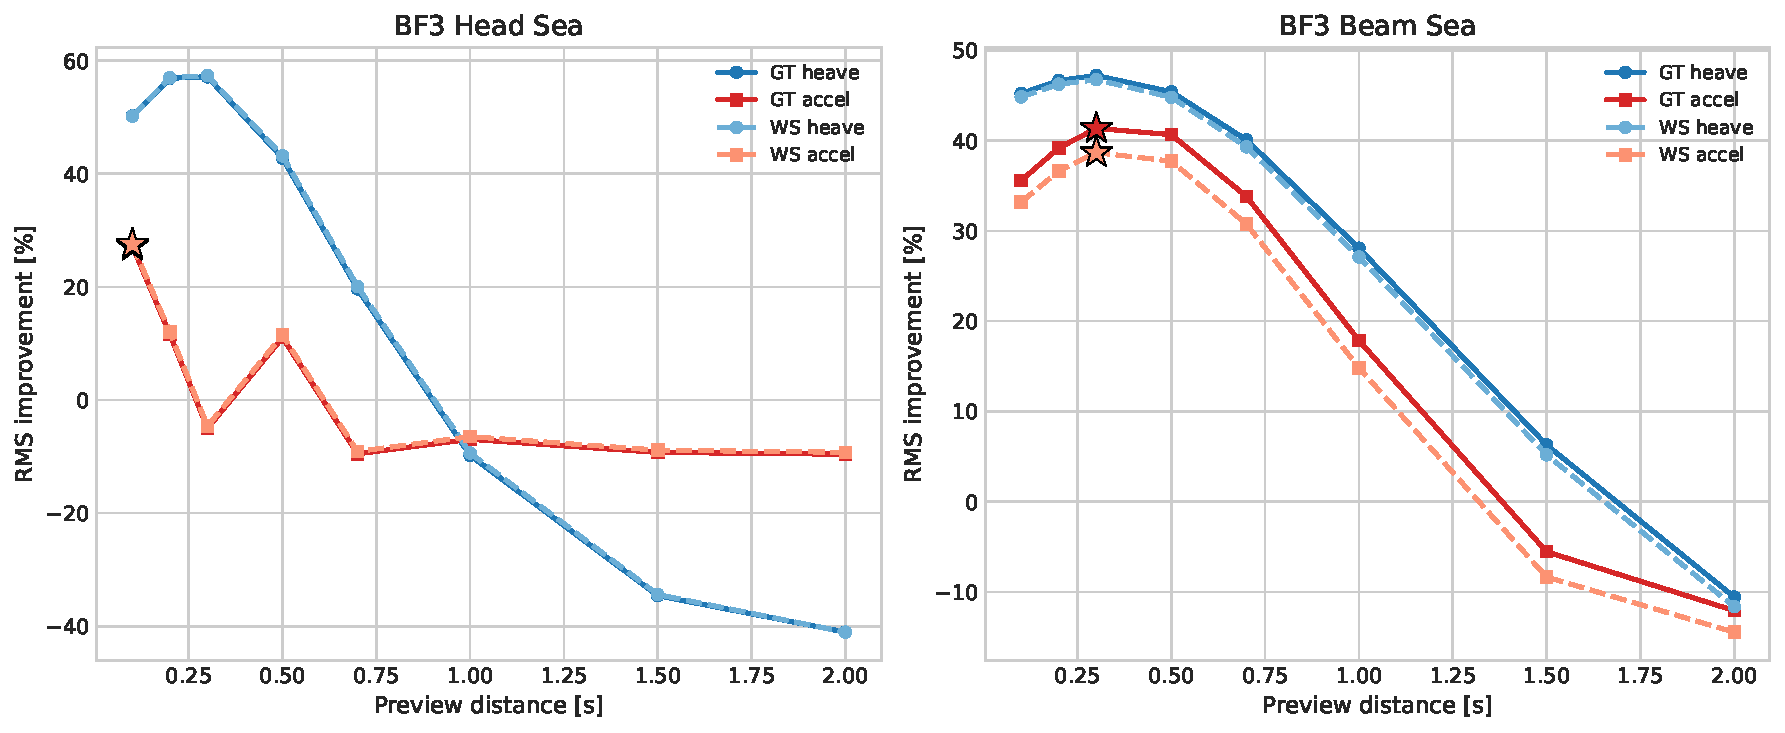
\includegraphics[width=0.80\textwidth]{figures_hf/fig_preview_sweep.pdf}
\caption{미리보기 거리($\Delta t_{\text{prev}}$)에 따른 가속도 개선율.
Head sea에서 0.1\,s, beam sea에서 0.3\,s가 최적이며,
장거리 미리보기는 파도 분산에 의해 성능이 저하된다.}
\label{fig:preview_sweep}
\end{figure}

최적 미리보기는 예상외로 짧다:
\begin{itemize}
  \item \textbf{Head sea}: 0.1\,s 최적 ($\sim$1.1\,m 전방) --- 높은 조우 주파수
        (22 knots BF3 head sea에서 Doppler 이동으로 $\sim$0.5\,Hz)로
        관련 파도 특징이 foil에 매우 가까이 위치.
  \item \textbf{Beam sea}: 0.3\,s 최적 ($\sim$3.4\,m 전방) --- 낮은 조우 주파수
        (Doppler 이동 없음)로 더 긴 유효 미리보기 창.
\end{itemize}

장거리 미리보기는 파도 분산과 다성분 간섭에 의한 공간 파도장 비상관화로
성능이 저하된다.
이 결과는 LiDAR 추정 시스템이 주로 각 foil 전방 $\sim$3\,m 이내의 근거리에서
정확해야 함을 의미하며, 이는 LiDAR 정밀도가 가장 높은 영역이다.

\subsection{LP 필터 파라미터}

$\alpha \in \{0.01, 0.03, 0.05, 0.10, 0.15, 0.20\}$ 스윕에서
$\alpha=0.05$가 4개 시나리오 중 3개에서 근최적 (최적 대비 2--3 pp 이내)이나,
BF4 Head에서 차선(최적 $\alpha=0.01$, +13.7\%; $\alpha=0.05$, +8.3\%)이다.
$\alpha \geq 0.15$에서 BF4 Head가 엄격히 해로워진다.
해상 상태 적응형 $\alpha$ 스케줄이 구체적 개선 경로이다.

\section{End-to-End 검증}
\label{sec:e2e}

시뮬레이션 LiDAR 에피소드에서 \WS{} 추정을 수행하고 추정된 스펙트럼 파라미터를
직접 feedforward 제어기에 투입하여 전체 파이프라인을 검증한다.
``Split'' 시뮬레이션: 해양은 GT 파도장에 의한 힘을 생성하고,
제어기는 \WS{} 추정만을 사용한다.

\begin{table}[htbp]
\centering
\caption{End-to-end 지연 시간 예산 (Intel i7-12700H, CPU 단일 스레드).}
\label{tab:latency}
\begin{tabular}{lcc}
\toprule
단계 & 지연 (ms) & 100\,ms 예산 대비 \\
\midrule
LiDAR 취득 (per scan, 10\,Hz) & 0.1 & 0.1\% \\
Point-cloud 전처리            & 0.5 & 0.5\% \\
\WS{} 추적 갱신            & 13.4 & 13.4\% \\
미리보기 평가 (4 foil points)   & 0.3 & 0.3\% \\
LP 필터 + feedforward 명령      & 0.2 & 0.2\% \\
PD 피드백 계산              & 0.1 & 0.1\% \\
\midrule
\textbf{총 파이프라인}              & \textbf{14.6} & \textbf{14.6\%} \\
\textbf{예산 여유}               & 85.4 & 85.4\% \\
\bottomrule
\end{tabular}
\end{table}

\begin{table}[htbp]
\centering
\caption{End-to-end \WS{} feedforward 결과.
$\Delta a$: PD-only 대비 가속도 RMS 개선. WS/GT: GT 개선 대비 \WS{} 달성 비율.}
\label{tab:e2e}
\begin{tabular}{lccc}
\toprule
에피소드 & GT $\Delta a$ & WS $\Delta a$ & WS/GT \\
\midrule
BF3 2-comp (단순)   & +35\% & +34\% & 96\% \\
BF3 5-comp (중간) & +38\% & +35\% & 92\% \\
BF4 5-comp (거친)    & +42\% & +16\% & 37\% \\
\bottomrule
\end{tabular}
\end{table}

\begin{figure}[htbp]
\centering
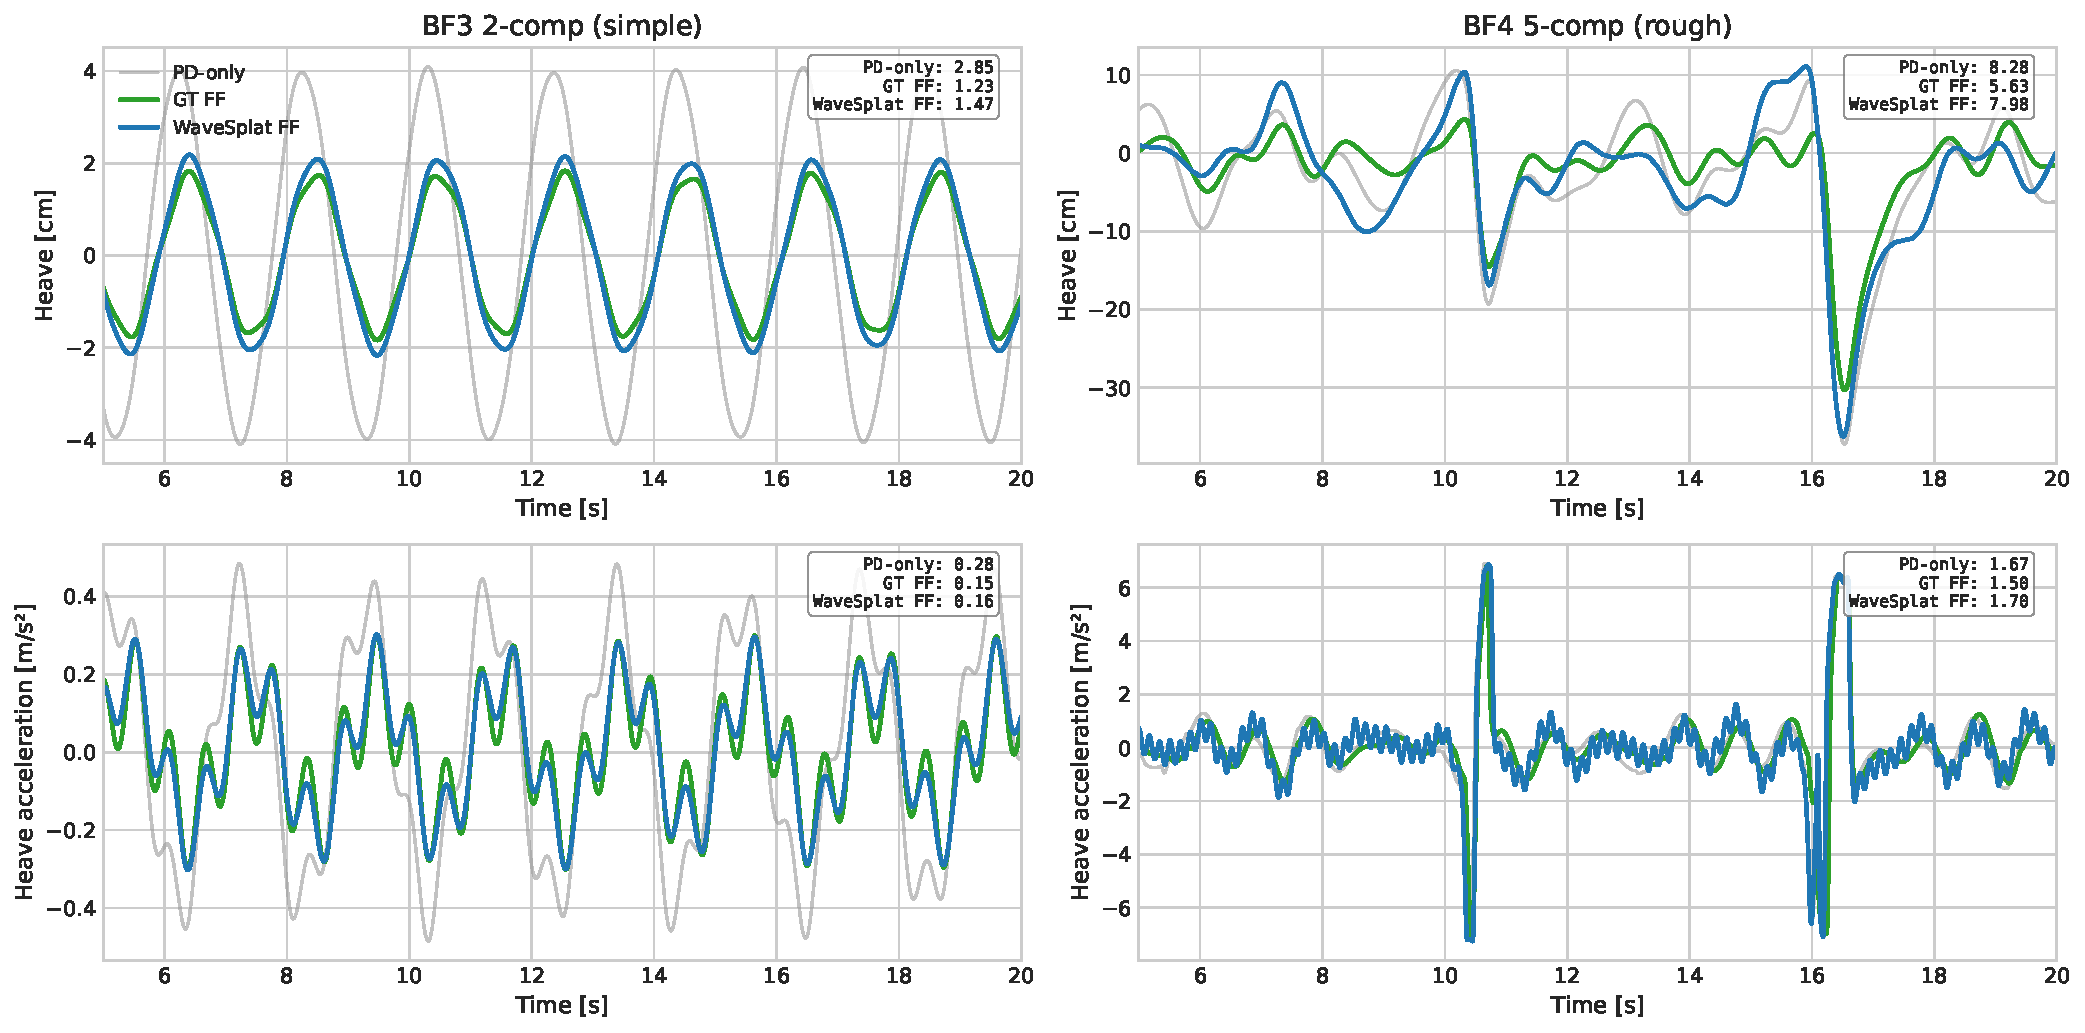
\includegraphics[width=0.95\textwidth]{figures_hf/fig_e2e_timeseries.pdf}
\caption{End-to-end 검증 시계열: BF3 2-component 에피소드.
상단: \WS{} 추정 파고 vs.\ ground truth. 하단: heave 가속도 비교
(PD-only, GT FF, \WS{} FF). \WS{} FF가 GT FF와 거의 동일한 가속도 저감을 달성한다.}
\label{fig:e2e_timeseries}
\end{figure}

\begin{figure}[htbp]
\centering
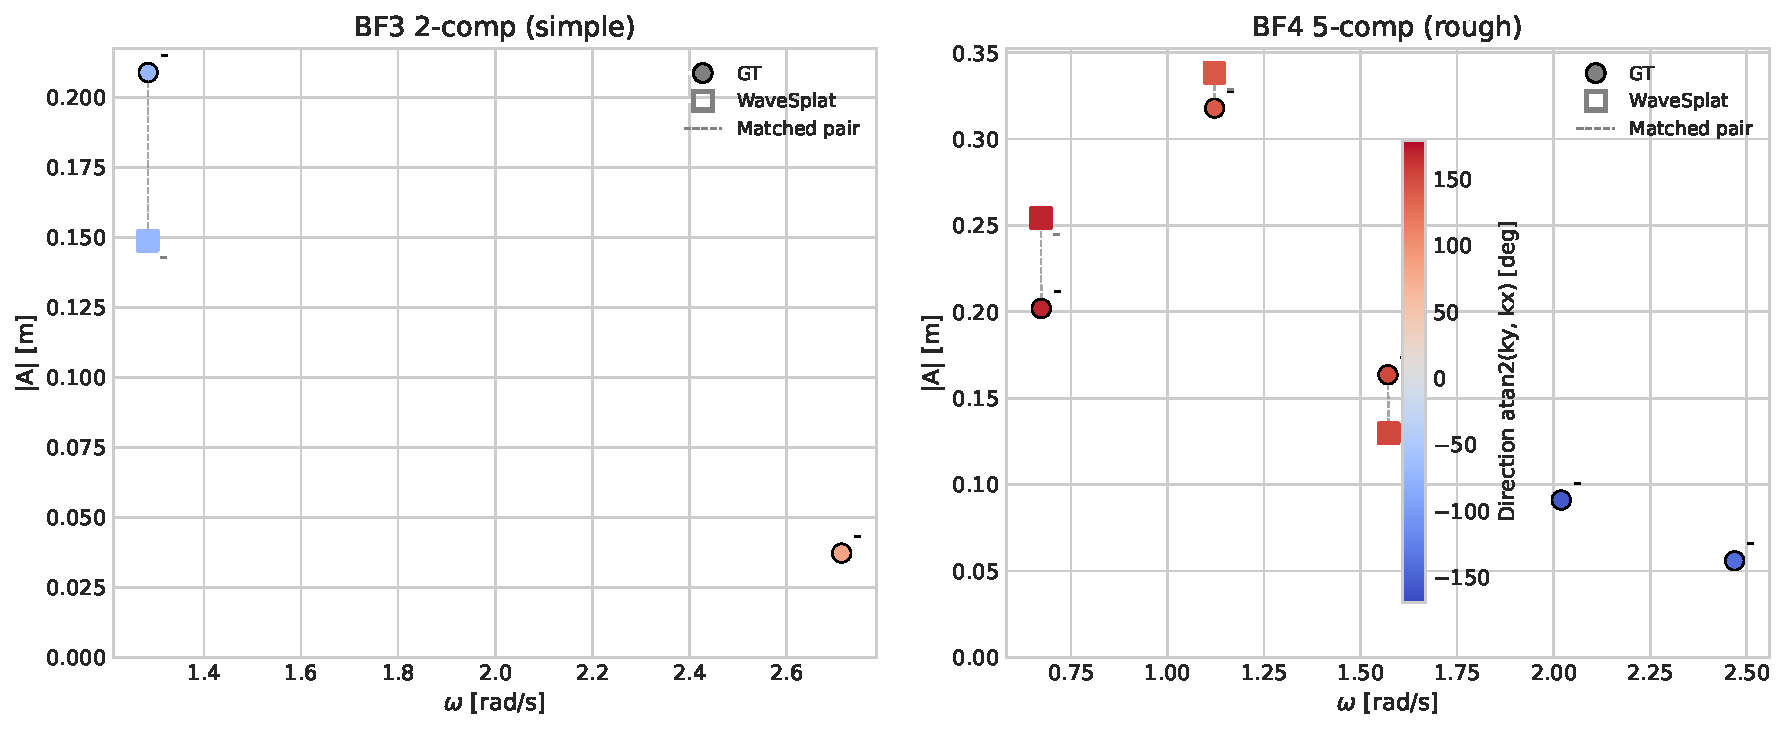
\includegraphics[width=0.80\textwidth]{figures_hf/fig_component_accuracy.pdf}
\caption{End-to-end 검증에서의 스펙트럼 성분 정확도.
\WS{}가 추정한 파수·진폭·위상과 ground truth의 비교.
BF3에서 지배 성분이 정확히 포착되나, BF4에서 일부 방향 오식별이 발생한다.}
\label{fig:component_accuracy}
\end{figure}

\textbf{BF3 (단순--중간 해상)}: \WS{}가 GT feedforward 이점의 92--96\%를 달성.
스펙트럼 추정이 2--5개 지배 성분을 정확히 포착하고, feedforward가
파도 유기 AoA 섭동을 효과적으로 선제 보상한다.
승차감이 ``Slight discomfort'' (PD-only, $a_\text{RMS} \approx 0.4$\,m/s$^2$)에서
``Comfortable'' (PD+WS FF, $a_\text{RMS} < 0.315$\,m/s$^2$)로 개선된다.

\textbf{BF4 (거친 해상)}: \WS{}가 GT의 37\%만 달성하여 현저히 저하된다.
추정된 vs.\ 실제 스펙트럼 성분 분석에서 원인이 밝혀진다:
\WS{}가 지배 파도 주파수와 진폭은 정확히 추정하나,
일부 성분의 전파 방향($k_x$ 부호)을 잘못 식별하여
feedforward 신호가 교란을 상쇄하지 않고 강화하는 결과를 낳는다.

\section{고찰}
\label{sec:hydrofoil_discussion}

\subsection{Feedforward가 하이드로포일에 효과적인 이유}

Feedforward 제어의 근본적 이점은 인과적 미리보기(causal preview)이다:
선박 전방의 파도장이 LiDAR 추정으로 관측 가능하므로, foil에 도달하기 전에
선제 대응할 수 있다.
20\% 추정 오차에서도, 저주파 파도 기울기와 궤도 속도 --- AoA 섭동의
지배적 기여 --- 가 효과적 선제 보상에 충분한 정밀도로 포착된다.

하이드로포일이 다른 선종보다 wave feedforward에 특히 적합한 이유:
(1) Foil이 고정 깊이에서 운용되어 파고/기울기와 양력 간의 직접적·거의 선형적 결합;
(2) 고순항 속도(22 knots)가 자연적 공간 미리보기를 제공;
(3) Foilborne 동역학의 낮은 감쇠로 비보상 파도 교란이 진동으로 지속;
(4) 스펙트럼 표현이 임의 공간 점에서 해석적 평가를 가능하게 하여
    격자 보간 오차를 제거.

\subsection{방향 추정의 중요성}

BF4 성능 저하 (WS/GT=37\%)는 방향 추정 정확도가 feedforward 응용에서
핵심적 병목임을 보여준다.
이는 제3장 6-지표 평가에서 \WS{}의 Dir $R^2 = -0.25$ (방향 추정이
chance 미만)와 일치한다.
$k_x$ 부호 오식별은 feedforward 신호의 부호를 반전시켜
교란을 강화하는 가장 치명적 추정 오차 유형이다.
진폭 오차는 feedforward 크기만 감소시키는 반면,
방향 오차는 이를 역전시킬 수 있다.

향후 개선 방향: 다중 프레임 방향 추적, feedforward 이득에서의
방향 신뢰도 가중치, 낮은 방향 신뢰도 성분에 대한 feedforward 차단(gating).

\subsection{한계}
\label{sec:hydrofoil_limits}

\begin{enumerate}
  \item \textbf{2DOF 단순화}: 롤 미포함. 비대칭 foil 설정의 beam sea에서
        중요할 수 있으며, 3DOF 확장은 port/starboard foil 차동 구동으로 구현 가능.
  \item \textbf{이상적 액추에이터}: 실제 foil flap 액추에이터의 유한 대역폭
        ($\sim$5--10\,Hz)과 속도 한계 미반영.
        Feedforward 신호 대역폭 ($<$1\,Hz)이 액추에이터 대역폭보다 충분히 낮아
        양호하나, 거친 해상에서의 combined feedback+feedforward 포화 가능성.
  \item \textbf{시뮬레이션 전용}: 간소화된 선박 모델. 물리적 하이드로포일 테스트베드
        검증이 필수.
  \item \textbf{시뮬레이션 길이}: 30초 에피소드. 60--120초의 장시간 시뮬레이션으로
        통계적 강건성과 추적 안정성의 추가 검증이 필요.
  \item \textbf{선박 파라미터 민감도}: 단일 대표 선박 설정만 사용.
        Feedforward 구조가 추정 파도 교란에 작용하므로 정성적 결론은
        일반화 가능하나, 정량적 가속도 저감은 선박별로 달라질 수 있음.
\end{enumerate}

% ============================================================================
% 제5장. 수조 실험 검증 (추후 추가)
% ============================================================================
\chapter{수조 실험 검증}
\label{chap:tank}

\todo{본 챕터는 조파수조 실험 완료 후 작성 예정.}

\noindent 계획 중인 내용:
\begin{itemize}
  \item \textbf{실험 설계}: 조파수조에서의 LiDAR 설치 조건 (높이, 각도, FOV 범위),
        파고계/용량식 센서 배치, JONSWAP 스펙트럼 기반 조파 조건 설정
  \item \textbf{Ground truth 확보}: 다중 용량식 파고계 어레이에 의한
        공간 분해 ground-truth 파고장 생성, 시간 동기화
  \item \textbf{Sim-to-Real gap 정량화}: 시뮬레이션(WaveSim)과 실제 LiDAR 관측 간의
        정량적 차이 분석 --- 노이즈 특성, raydrop 패턴, 다중 경로 반사 등
  \item \textbf{\WS{} 실제 데이터 적용}: 시뮬레이션에서 개발된 \WS{}를
        실제 LiDAR 데이터에 직접 적용하여 6-지표 패널로 성능 평가
  \item \textbf{튜닝 필요성 분석}: 시뮬레이션 최적 하이퍼파라미터가 실데이터에서도
        유효한지, 또는 재튜닝이 필요한지 평가
\end{itemize}

% ============================================================================
% 제6장. 결론 및 향후 연구
% ============================================================================
\chapter{결론 및 향후 연구}
\label{chap:conclusion}

\section{결론}
\label{sec:conclusion}

본 논문은 희소 선박 탑재 LiDAR 관측으로부터 실시간 파도장을 추정하는
격자 비의존 스펙트럼 Gaussian 방법 \WS{}를 제안하고,
이를 하이드로포일 선박의 파랑 예측 기반 feedforward 제어에 응용하였다.
주요 결론은 다음과 같다:

\paragraph{파도장 추정 (\WS{})}
파도장을 $N$개의 평면파 집합으로 파라미터화하고
분산관계를 하드 제약으로 부과한 격자 비의존 스펙트럼 추정 프레임워크를 제안하였다.
100 에피소드 평가에서 24개 설정으로 최적화된 ETKF 대비
nRMSE를 \textbf{30.1\%} 낮추고 (\textbf{0.223} vs.\ 0.319),
약 \textbf{10배} 빠른 처리 속도 (\textbf{13.4} vs.\ 132.6\,ms/프레임)를 달성하였다.
사전 등록된 6-지표 패널에서 \WS{}는 zero-predictor 대비 양수의
Skill Score를 기록한 유일한 방법이었으며,
이 6-지표 패널은 ETKF의 ``분산 정합이나 형상 불일치'' (VR=0.90, $\rho$=0.11)와
GPR의 ``near-zero predictor'' (VR=0.065) 실패 모드를 nRMSE 단독으로는
드러나지 않는 진단적 가치를 입증하였다.
100회 대응 검증 (Wilcoxon $p = 1.1\times10^{-15}$, Cohen's $d = 1.16$)으로
이 차이가 통계적으로 large effect임을 확인하였다.

적응형 모델 차수는 단순 너울($N=1$)에서 복잡한 다성분 해상($N=21$)까지
자동 적응하여 고정 $N=15$ 대비 6.4\% 추가 개선을 달성하였다.
두 가지 LiDAR raydrop 모델(확산/specular)과 20\% 관측 밀도에서도
견고한 성능을 보였으며, 추가 노이즈 주입(기준선 5배)에서도
$\pm$13\% 이내의 안정적 성능을 유지하였다.

\paragraph{하이드로포일 Feedforward 제어}
\WS{}의 스펙트럼 파도장 추정을 활용하는 dual-actuator wave-preview feedforward
제어를 제안하였다. IIR 저역통과 필터($\alpha=0.05$)가 추정 노이즈를 억제하면서
파도 미리보기 신호를 보존하는 설계로,
Beaufort 3--4 조건에서 heave 가속도 RMS를 11--41\% 감소시켰다.
End-to-end 검증에서 \WS{} 기반 feedforward는 BF3에서
GT 대비 92--96\%의 성능을 달성하였으며,
ISO 2631 승차감을 ``Slight discomfort''에서 ``Comfortable''로 개선하였다.

민감도 분석에서 feedforward는 50\% nRMSE까지도 효과적임이 확인되어,
파도 추정 시스템이 매우 높은 정밀도를 요구하지 않음을 보였다.
최적 미리보기 거리는 0.1--0.3초(1--3\,m)로 짧아,
LiDAR 정밀도가 가장 높은 근거리 영역과 일치한다.

방향 추정 정확도가 feedforward 성능의 핵심 병목임이 밝혀졌다
(BF4에서 WS/GT=37\%, Dir $R^2=-0.25$에 기인).
이는 \WS{}의 가장 중요한 개선 방향을 제시한다.

전체 파이프라인(LiDAR $\to$ \WS{} $\to$ feedforward)의 지연은
14.6\,ms/cycle로 100\,ms 실시간 예산의 14.6\%만 소비하여,
표준 선박 탑재 컴퓨팅 하드웨어에서의 실용적 배치가 가능하다.

\section{향후 연구}
\label{sec:future_work}

\begin{enumerate}
  \item \textbf{수조 실험 검증}: 조파수조에서 LiDAR + \WS{} 적용,
        파고계 기반 ground truth와의 비교를 통한 Sim-to-Real gap 정량화.
        시뮬레이션에서 확인된 39개 물리 단위 테스트의 실데이터 대응 검증.

  \item \textbf{방향성 추정 개선}: Dir $R^2 = -0.25$의 한계를 극복하기 위한
        방향 추정 알고리즘 개선. 다중 프레임 방향 추적,
        3D $(k_x, k_y, \omega)$ FFT 기반 초기화, 또는
        방향 von Mises 기저함수 도입 검토.

  \item \textbf{비선형 파도 모델}: Stokes 2차 이상의 비선형 항을 포함하는
        forward 모델 확장. 스펙트럼 파라미터화를 유지하면서
        가파른 파도에서의 모델 불일치를 줄인다.

  \item \textbf{해류 추정 통합}: 해류 성분을 파라미터에 포함한 통합 추정.
        Doppler 이동 $\omega = \sqrt{g|k|\tanh(|k|d)} + \mathbf{k}\cdot\mathbf{U}$의
        해류 벡터 $\mathbf{U}$를 동시 추정.

  \item \textbf{MPC 기반 6DOF 제어}: \WS{} 예측값을 활용하는
        Model Predictive Control 확장. 액추에이터 제약
        ($\pm 15^\circ$ 플랩 한계)을 명시적으로 처리하고,
        거친 해상에서의 최적 제어를 달성.
        롤 자유도 추가로 beam sea 롤 제어 구현.

  \item \textbf{방향 신뢰도 기반 feedforward 게이팅}: 낮은 방향 신뢰도의
        스펙트럼 성분에 대한 feedforward 권한을 감소시켜,
        방향 오식별에 의한 feedforward 역전을 방지.
        완벽한 방향 추정 없이도 BF4 성능을 개선할 수 있는 실용적 경로.
\end{enumerate}

% ============================================================================
% 참고문헌
% ============================================================================
\newpage
\bibliographystyle{elsarticle-harv}
\bibliography{thesis_refs}

% ============================================================================
% 감사의 글
% ============================================================================
\chapter*{감사의 글}
\addcontentsline{toc}{chapter}{감사의 글}

\todo{감사의 글 작성}

\end{document}
